%% bare_conf.tex
%% V1.4b
%% 2015/08/26
%% by Michael Shell
%% See:
%% http://www.michaelshell.org/
%% for current contact information.
%%
%% This is a skeleton file demonstrating the use of IEEEtran.cls
%% (requires IEEEtran.cls version 1.8b or later) with an IEEE
%% conference paper.
%%
%% Support sites:
%% http://www.michaelshell.org/tex/ieeetran/
%% http://www.ctan.org/pkg/ieeetran
%% and
%% http://www.ieee.org/

%%*************************************************************************
%% Legal Notice:
%% This code is offered as-is without any warranty either expressed or
%% implied; without even the implied warranty of MERCHANTABILITY or
%% FITNESS FOR A PARTICULAR PURPOSE! 
%% User assumes all risk.
%% In no event shall the IEEE or any contributor to this code be liable for
%% any damages or losses, including, but not limited to, incidental,
%% consequential, or any other damages, resulting from the use or misuse
%% of any information contained here.
%%
%% All comments are the opinions of their respective authors and are not
%% necessarily endorsed by the IEEE.
%%
%% This work is distributed under the LaTeX Project Public License (LPPL)
%% ( http://www.latex-project.org/ ) version 1.3, and may be freely used,
%% distributed and modified. A copy of the LPPL, version 1.3, is included
%% in the base LaTeX documentation of all distributions of LaTeX released
%% 2003/12/01 or later.
%% Retain all contribution notices and credits.
%% ** Modified files should be clearly indicated as such, including  **
%% ** renaming them and changing author support contact information. **
%%*************************************************************************


% *** Authors should verify (and, if needed, correct) their LaTeX system  ***
% *** with the testflow diagnostic prior to trusting their LaTeX platform ***
% *** with production work. The IEEE's font choices and paper sizes can   ***
% *** trigger bugs that do not appear when using other class files.       ***                          ***
% The testflow support page is at:
% http://www.michaelshell.org/tex/testflow/



\documentclass[conference]{IEEEtran}
% Some Computer Society conferences also require the compsoc mode option,
% but others use the standard conference format.
%
% If IEEEtran.cls has not been installed into the LaTeX system files,
% manually specify the path to it like:
% \documentclass[conference]{../sty/IEEEtran}





% Some very useful LaTeX packages include:
% (uncomment the ones you want to load)


% *** MISC UTILITY PACKAGES ***
%
%\usepackage{ifpdf}
% Heiko Oberdiek's ifpdf.sty is very useful if you need conditional
% compilation based on whether the output is pdf or dvi.
% usage:
% \ifpdf
%   % pdf code
% \else
%   % dvi code
% \fi
% The latest version of ifpdf.sty can be obtained from:
% http://www.ctan.org/pkg/ifpdf
% Also, note that IEEEtran.cls V1.7 and later provides a builtin
% \ifCLASSINFOpdf conditional that works the same way.
% When switching from latex to pdflatex and vice-versa, the compiler may
% have to be run twice to clear warning/error messages.

\usepackage[english]{babel}
\usepackage{blindtext}
\usepackage{xcolor}
%\usepackage[hidelinks]{hyperref}        % interne Hyperlinks
\usepackage[utf8]{inputenc}
\usepackage{amsmath}
\usepackage{amsfonts}
\usepackage{amssymb}
\usepackage{tikz}
\usepackage[hang]{footmisc}
\usepackage{booktabs}
\usepackage{multirow}
\usepackage[all=normal,mathspacing=tight,wordspacing=tight,tracking=normal,charwidths=tight,mathdisplays=normal,paragraphs=tight,bibbreaks=tight,floats=tight]{savetrees}

\usetikzlibrary{arrows,chains,matrix,positioning,scopes,shapes.geometric}
\definecolor{myblue}{HTML}{004A99}

\renewcommand{\baselinestretch}{0.95} 

%Mathdisplays tighter spacing:
\AtBeginDocument{%
	\abovedisplayskip=3pt plus 3pt	
	\belowdisplayskip=3pt plus 3pt	
	\abovedisplayshortskip=0pt plus 0pt	
	\belowdisplayshortskip=0pt plus 0pt	
}
\DeclareMathOperator{\lcm}{lcm}
\setlength{\skip\footins}{0.1cm}

%Footnode indent
\makeatletter
\newcommand{\specificthanks}[1]{\@fnsymbol{#1}}% Inserts a specific \thanks symbol
\renewcommand\@makefntext[1]{%
	\@setpar{%
		\@@par \@tempdima=\hsize
		\advance\@tempdima by -0.4cm\relax
		\parshape \@ne 0.4cm \@tempdima
	}%
	\par \parindent=\z@ \noindent
	\hb@xt@ \z@{\hss \hb@xt@ 0.4cm\textsuperscript{\@thefnmark\hss}}%
	#1%
}
\makeatother


% *** CITATION PACKAGES ***
%
%\usepackage{cite}
% cite.sty was written by Donald Arseneau
% V1.6 and later of IEEEtran pre-defines the format of the cite.sty package
% \cite{} output to follow that of the IEEE. Loading the cite package will
% result in citation numbers being automatically sorted and properly
% "compressed/ranged". e.g., [1], [9], [2], [7], [5], [6] without using
% cite.sty will become [1], [2], [5]--[7], [9] using cite.sty. cite.sty's
% \cite will automatically add leading space, if needed. Use cite.sty's
% noadjust option (cite.sty V3.8 and later) if you want to turn this off
% such as if a citation ever needs to be enclosed in parenthesis.
% cite.sty is already installed on most LaTeX systems. Be sure and use
% version 5.0 (2009-03-20) and later if using hyperref.sty.
% The latest version can be obtained at:
% http://www.ctan.org/pkg/cite
% The documentation is contained in the cite.sty file itself.



% *** PDF, URL AND HYPERLINK PACKAGES ***
%
%\usepackage{url}
% url.sty was written by Donald Arseneau. It provides better support for
% handling and breaking URLs. url.sty is already installed on most LaTeX
% systems. The latest version and documentation can be obtained at:
% http://www.ctan.org/pkg/url
% Basically, \url{my_url_here}.




% correct bad hyphenation here
\hyphenation{op-tical net-works semi-conduc-tor}


\begin{document}
%
% paper title
% Titles are generally capitalized except for words such as a, an, and, as,
% at, but, by, for, in, nor, of, on, or, the, to and up, which are usually
% not capitalized unless they are the first or last word of the title.
% Linebreaks \\ can be used within to get better formatting as desired.
% Do not put math or special symbols in the title.
%\title{System Synthesis using Answer Set Programming Modulo Theories}
\title{Enhancing Symbolic System Synthesis through ASPmT with Partial Assignment Evaluation}


% author names and affiliations
% use a multiple column layout for up to three different
% affiliations
%\author{\IEEEauthorblockN{Kai Neubauer, Christian Haubelt}
%\IEEEauthorblockA{University of Rostock\\Rostock, Germany\\
%\{kai.neubauer, christian.haubelt\}@uni-rostock.de}
%\and
%\IEEEauthorblockN{Philipp Wanko, Torsten Schaub}
%\IEEEauthorblockA{University of Potsdam\\
%Potsdam, Germany\\
%\{wanko, torsten\}@cs.uni-potsdam.de}}
\author{
	Kai Neubauer\textsuperscript{\specificthanks{1}}, Philipp Wanko\textsuperscript{\specificthanks{2}}, Torsten Schaub\textsuperscript{\specificthanks{2}}, and Christian Haubelt\textsuperscript{\specificthanks{1}}
	\\\small{\textsuperscript{\specificthanks{1}}University of Rostock, Applied Microelectronics and Computer Engineering, Germany}
	\\\small{\textsuperscript{\specificthanks{2}}University of Potsdam, Knowledge Processing and Information Systems, Germany}
	\\\footnotesize{\{kai.neubauer,christian.haubelt\}@uni-rostock.de}, \{wanko, torsten\}@cs.uni-potsdam.de%\vspace*{-3mm}
	%\\ % To make more spaces just add \\!
}
%\author{\IEEEauthorblockN{Blinded}
%\IEEEauthorblockA{Blinded\\blinded\\
%blinded@blinded.blinded}}
%\and
%\IEEEauthorblockN{James Kirk\\ and Montgomery Scott}
%\IEEEauthorblockA{Starfleet Academy\\
%San Francisco, California 96678--2391\\
%Telephone: (800) 555--1212\\
%Fax: (888) 555--1212}}

% conference papers do not typically use \thanks and this command
% is locked out in conference mode. If really needed, such as for
% the acknowledgment of grants, issue a \IEEEoverridecommandlockouts
% after \documentclass

% for over three affiliations, or if they all won't fit within the width
% of the page, use this alternative format:
% 
%\author{\IEEEauthorblockN{Michael Shell\IEEEauthorrefmark{1},
%Homer Simpson\IEEEauthorrefmark{2},
%James Kirk\IEEEauthorrefmark{3}, 
%Montgomery Scott\IEEEauthorrefmark{3} and
%Eldon Tyrell\IEEEauthorrefmark{4}}
%\IEEEauthorblockA{\IEEEauthorrefmark{1}School of Electrical and Computer Engineering\\
%Georgia Institute of Technology,
%Atlanta, Georgia 30332--0250\\ Email: see http://www.michaelshell.org/contact.html}
%\IEEEauthorblockA{\IEEEauthorrefmark{2}Twentieth Century Fox, Springfield, USA\\
%Email: homer@thesimpsons.com}
%\IEEEauthorblockA{\IEEEauthorrefmark{3}Starfleet Academy, San Francisco, California 96678-2391\\
%Telephone: (800) 555--1212, Fax: (888) 555--1212}
%\IEEEauthorblockA{\IEEEauthorrefmark{4}Tyrell Inc., 123 Replicant Street, Los Angeles, California 90210--4321}}


%\IEEEspecialpapernotice{(Invited Paper)}

\maketitle

\newcommand{\gringo}{\textit{gringo}}
\newcommand{\clasp}{\textit{clasp}}
\newcommand{\clingo}{\textit{clingo}}
\newcommand{\asprin}{\textit{asprin}}
\newcommand{\asap}{\textit{teaspoon}}
\newcommand{\piclasp}{\textit{piclasp}}

\newcommand{\code}[1]{\lstinline[basicstyle=\ttfamily]{#1}}

\newcommand{\lw}[1]{\smash{\lower1.ex\hbox{#1}}}
\newcommand{\llw}[1]{\smash{\lower3.ex\hbox{#1}}}

%\newcommand{\dataCL}[5]{%
%  \code{#1} & #3 & #5 & #4
%}
%\newcommand{\dataCS}[5]{%
%  #3 & #5 & #4
%}

\newenvironment{tableC}{%
  \scriptsize
  \tabcolsep = 0.6mm
  \begin{tabular}[t]{l|rlr|rlr|rlr|rlr|rlr}\hline
    \multicolumn{1}{l|}{\llw{Instance}} &
    \multicolumn{3}{c|}{UD1} &
    \multicolumn{3}{c|}{UD2} &
    \multicolumn{3}{c|}{UD3} &
    \multicolumn{3}{c|}{UD4} &
    \multicolumn{3}{c}{UD5} \\
    & 
    \multicolumn{1}{c}{Best} & & \multicolumn{1}{c|}{\emph{tea-}} & 
    \multicolumn{1}{c}{Best} & & \multicolumn{1}{c|}{\emph{tea-}} & 
    \multicolumn{1}{c}{Best} & & \multicolumn{1}{c|}{\emph{tea-}} & 
    \multicolumn{1}{c}{Best} & & \multicolumn{1}{c|}{\emph{tea-}} & 
    \multicolumn{1}{c}{Best} & & \multicolumn{1}{c}{\emph{tea-}} \\
    & 
    known & & \emph{spoon} & 
    known & & \emph{spoon} & 
    known & & \emph{spoon} & 
    known & & \emph{spoon} & 
    known & & \emph{spoon} \\
    \hline
  }{%
    \hline
  \end{tabular}
}

\newenvironment{tableB}{%
  \scriptsize
  \tabcolsep = 0.7mm
%  \begin{tabular}[t]{|l|c|r|l|l|l|}\hline
  \begin{tabular}[t]{lcrlll}\hline
    Instance &
    Formulation &
    Time (sec.)\\
    \hline
  }{%
    \hline
  \end{tabular}
}
\newenvironment{tableL}{%
  \scriptsize
  \tabcolsep = 0.7mm
  \begin{tabular}[t]{l|rrrrrrrr|r}\hline
    \lw{Instance} &
    \lw{Time (sec.)} &
    \multicolumn{6}{c}{The best utility vector} &
    The sum of  &
    The best of basic\\
    &
    &
    $(S_1,$ & $S_4,$ & $S_2,$ & $S_7,$ & $S_6,$ & $S_3)$ &
    utility vector &
    and optimized \\
    \hline
  }{%
    \hline
  \end{tabular}
}

%%% Local Variables:
%%% mode: latex
%%% TeX-master: "paper"
%%% End:


%\begin{abstract}
%	The design space for highly complex system level specifications of embedded systems is enormous as tasks may be mapped to different resources and messages may be routed over several links of the hardware platform. 
%	Furthermore, highly constrained requirements lead to many infeasible solutions that have to be sorted out. \emph{\ac{ASP}} in combination with variant background theories (\emph{\ac{ASPmT}}) has been shown to cope with such requirements very efficiently. However, especially in system level design, a fast \emph{\ac{DSE}} including optimization is crucial in order to steer the development towards optimal design points. In this paper, we therefore propose to couple the highly efficient constraint solving capabilities of \ac{ASP} with a \ac{DSE} including \emph{multi-objective optimization} in an additional background theory. Utilizing the possibility to work on \emph{partial assignments}, \ac{ASPmT} is able to prune entire infeasible and dominated regions from the search space early in the decision process. In the experimental section, we present and compare variant approaches and domain specific heuristics.
%\end{abstract}

\begin{abstract}
	An efficient \emph{\ac{DSE}} is imperative for the design of modern, highly complex embedded systems in order to steer the development towards optimal design points. The early evaluation of design decisions at system-level abstraction layer helps to find promising regions for subsequent development steps in lower abstraction levels by diminishing the complexity of the search problem. In recent works, symbolic techniques, especially \ac{ASPmT}, have been shown to find feasible solutions of highly complex system-level synthesis problems with non-linear constraints very efficiently. In this paper, we present a novel approach to a holistic system-level \ac{DSE} based on \ac{ASPmT}. To this end, we include additional background theories that concurrently guarantee compliance with hard constraints and perform the simultaneous optimization of several design objectives. %First experimental results show the applicability of our approach. %for large optimization of up to 170 tasks mapped to 3-dimensional hardware platforms. Furthermore, it outperforms current multi-objective optimization strategies of \ac{ASP} with respect to both diversity and convergence of found solutions.   %We present and investigate several strategies that show the applicability of our approach even for large problem instances. 
	We implement and compare our approach with a state-of-the-art preference handling framework for \ac{ASP}. Experimental results indicate that our proposed method produces better solutions with respect to both diversity and convergence to the true Pareto front.
\end{abstract}

% no keywords




% For peer review papers, you can put extra information on the cover
% page as needed:
% \ifCLASSOPTIONpeerreview
% \begin{center} \bfseries EDICS Category: 3-BBND \end{center}
% \fi
%
% For peerreview papers, this IEEEtran command inserts a page break and
% creates the second title. It will be ignored for other modes.
\IEEEpeerreviewmaketitle

\section{Introduction and Related Work}
With the ever growing demand for highly complex embedded systems in both industrial and consumer environments, efficient design techniques gain progressively more importance. 
To satisfy the requested productivity constraints, the abstraction of embedded systems design has been raised to the electronic system level. 
In system synthesis, a task-level behavioral description is transformed into a structural representation considering certain constraints such as available computational (CPUs, DSPs,  hardware accelerators) and communication (buses, routers) resources as well as extra-functional requirements \cite{Gerstlauer2009}. \par
To perform a holistic synthesis, resources have to be selected from an architectural template, 
computational tasks and messages have to be mapped onto computational resources and routed over the allocated communication infrastructure, respectively, and finally, 
a schedule has to be determined that complies with given timing constraints like latency or throughput requirements.\par
In order to cope with the ever increasing complexity of functional and non-functional requirements of embedded systems, 
symbolic techniques have traditionally been employed in embedded system synthesis since the early 2000s, e.g. \cite{Haubelt2003,Lukasiewycz2009,Lukasiewycz2012}. 
While the encoding of feasible mapping and routing decisions into Boolean formulas led to efficient synthesis frameworks by leveraging enhancements in state-of-the-art Boolean satisfiability (SAT) solvers, 
numerical and non-linear problems (such as scheduling) are not easily representable in Boolean logic. 
As a consequence, SMT-based techniques, i.e. the combination of Boolean logic (traditionally SAT) and variant background theories, have been developed in the domain of embedded systems synthesis \cite{Satish2007,Reimann2010,Andres2015,Biewer2015,Liu2011}. 
In one of the first works on SMT-based approaches, Reimann et al.\ \cite{Reimann2010} integrate a background theory solver to evaluate partial assignments of an underlying SAT-solver. 
In contrast to the work at hand, the authors do not consider scheduling decisions. 
In \cite{Reimann2011}, they extend their approach to constructing schedules though only consider complete assignments, i.e.\ mapping and routing is already completed.\par
The authors of \cite{Liu2011} present another SMT-based method for scheduling analysis in a background theory. 
Similar to the proposed approach in this paper, they utilize \emph{quantifier free integer difference logic} (QF--IDL) as background theory to identify valid schedules. 
The main advantages of QF--IDL are its decidability in polynomial time%\footnote{Note that the overall system synthesis problem is $\mathcal{NP}$--hard.} 
~\cite{Sebastiani2007} and the possibility to leverage the solving process to directly analyze and propagate observed conflicts. 
Yet, the work of \cite{Liu2011} does not support cyclic or periodic applications nor heterogeneous architectures whereas our approach considers a much more sophisticated system model allowing us to synthesize cyclic and periodic behavior.
%While the approach in \cite{Liu2011} only considers acyclic and aperiodic applications as well as homogeneous hardware architectures, our work provides a more sophisticated system model as it supports additionally cyclic and periodic applications that may be implemented on heterogeneous architectures. 
%While they also utilize QF--IDL, they do not support cyclic and periodic applications nor heterogeneous architectures. 
\par The work of Andres and Biewer et al. in \cite{Andres2015} and \cite{Biewer2015} is the most related to our approach. 
They suggest to replace the SAT-solver with an \emph{answer set programming} (ASP) solver as it has been shown to decide routing options more efficiently. 
To analyze timing constraints, they use separate ASP and QF--IDL-based SMT-solvers which communicate indicator variables through a shared text file. 
Thus, in this configuration, an evaluation of partial assignments is not supported.
%Furthermore, the applications considered in \cite{Andres2015} and \cite{Biewer2015} only contain simple linear dependencies and assume the deadline of applications to match their period. 
Furthermore, the system model considered in \cite{Andres2015} and \cite{Biewer2015} is very restrictive. It only allows the representation of simple linear applications where deadlines of tasks have to be smaller than their corresponding periods. 
In combination with a homogeneous hardware architecture and unconstrained mapping options, the authors are able to exploit symmetries in the synthesis problem and use advanced heuristics which simplifies the solving accordingly.

\textbf{Contributions:} In this paper, we first present a mathematical formulation that allows us to describe more sophisticated system models for streaming applications on heterogeneous hardware architectures compared to previous work. 
In particular, this includes deadline-constrained periodic and cyclic applications. Second, we integrate the background theory \emph{QF--IDL} directly into the state-of-the-art ASP-Solver \emph{clingo} \cite{gekakaosscwa16a} which results in a much tighter coupling between background and foreground theories. Third, individual propagators check extra-functional constraints early in the decision process by utilizing \emph{partial assignment checking}. Thus, large infeasible areas of design points can be excluded from the search space more efficiently.

\textbf{Paper organization: } 
In Sec.~\ref{sec:model}, a detailed presentation of the underlying specification model is given. 
The proposed synthesis framework including binding, routing, and scheduling encodings as well as first results are presented in Sec.~\ref{sec:synthesis}. 
Finally, Sec.~\ref{sec:conclusion} concludes this work and discusses future challenges. 
%\newpage

%\section{Introduction}
\label{sec:introduction}
%In order to cope with the ever-increasing complexity of embedded systems, system level description are utilized to diminish the complexity of finding potentially good solutions which can then be used as initial starting points for further optimization in lower abstraction levels. On system level, applications are composed of granular tasks that exchange information over communication messages and form dependency relations between each other. The hardware architecture contains heterogeneous processing elements (e.g.~CPU, DSP, GPU) as well as a communication infrastructure like routers and links. Yet, the design space for such system level specifications of embedded systems is still enormous as tasks may be mapped to different computational resources and messages may be routed over several links of the communication infrastructure.\par 
%Furthermore, various hard constraints like maximum latency and energy consumption of the resulting systems have to be considered. That is, only a subset of all possible decisions leads to valid system implementations that conform to previously defined constraints which makes it even hard\footnote{In fact, the mapping problem is known to be $\mathcal{NP}$-hard \cite{Blickle1998}.} to find \emph{one} feasible solution. However, by encoding the problem symbolically (cf.~\cite{Haubelt2003}) and due to the technological advances in \ac{SAT}, various constraint solvers can be utilized to cope with the complexity. Especially, \emph{\acf{ASP}} has been shown to deal with such stringently constrained design problems very efficiently (e.g.~\cite{Andres2013}). Opposed to other symbolic techniques like \ac{SAT}, reachability can be expressed naturally in \ac{ASP} which fastens the routing sub-problem.\par 
%%\ac{ASP} stems from the area of knowledge representation and reasoning and is based on the \emph{stable model semantics}. 
%Finding one feasible solution is however often insufficient. Depending on the decisions that have been made, the qualitative properties (e.g.~latency, energy consumption, area requirements) of the resulting system implementation may vary considerably from solution to solution. Thus, a \acf{DSE} is imperative to find solutions with optimal properties. Usually, the objectives (i.e.~optimizing the individual properties) of \acp{MOOP} are conflicting with each other and no single optimal solution but a set of \emph{Pareto optimal} solutions exists. A Pareto optimal solution is characterized by the property that it is not dominated by (i.e.~not worse in all objectives than) any other solution. \par%That is, all Pareto optimal solutions are mutually non-dominated.\par 
%Commonly, meta-heuristics like \acp{MOEA} are utilized to solve \acp{MOOP}. They are based on natural processes and work on sets of solutions (populations) concurrently. Each solution is evaluated by a fitness function with respect to the objectives and the best solutions are combined to create novel solutions for subsequent generations. As the initial population is created by a randomized process, finding feasible solutions becomes a problem for stringently constraint environments. Moreover, because the search is generally not executed systematically but based on combining previously found solutions, \acp{MOEA} tend to run into saturation and stop finding novel solutions after an arbitrary number of iterations.\par
%In the paper at hand, we therefore propose an approach that utilizes an exact symbolic encoding for both the constraint solving and the design space exploration. Based on \ac{ASP}, we tightly integrate background theory solvers, known as \ac{ASPmT}, that handle (non-)linear objectives as well as Pareto filtering of found solutions. Furthermore, they are able to work on partial solutions to prune the search space from infeasible and dominated regions of design points early in the decision process. 
%The contribution of this paper is threefold:
%\begin{enumerate}
%	\item We present a universal framework for preference handling that is capable of both linear and non-linear objectives based on \ac{ASPmT}.
%	\item In order to combine various background theories for multi-objective optimization and constraint solving concurrently, we present various approaches.
%	\item Extensive experimental test instances show the advantages and disadvantages of the different approaches. 
%\end{enumerate}\par
%\textbf{Paper organization:} Related work will be covered in Sec.~\ref{sec:relatedwork}. Afterwards, the execution model that will be used throughout the paper is briefly described in Sec.~\ref{sec:model}. Section \ref{sec:framework} contains detailed information about our proposed preference handling framework. Experimental results are given in Sec.~\ref{sec:experiments} before Sec.~\ref{sec:conclusion} concludes the paper.

%Essentially, there are three approaches to explore the design space \cite{Pimentel2017}: First, meta-heuristics like evolutionary algorithms have been studied thoroughly in the past (e.g.~\cite{1,2,3,4,5}). Those techniques are inspired by the natural selection process and work on whole sets of solutions (populations) concurrently. Each solution is evaluated and the best are combined to create new solutions for the following generations. One major problem arises if, due to various hard constraints, only a small subset of design points is feasible. Because of their random nature, pure meta-heuristics tend to fail in finding feasible regions of the design space. \par 
%Therefore, the second approach type combines meta-heuristics with exact methods (e.g.~\cite{Neubauer2016,Haubelt2003,Lukasiewycz2012a}). That is, not the decision variables themselves but the heuristics that are used by the constraint solver are subject to the randomized exploration process. Every found design point is thereby guaranteed to be feasible.\par 
%Finally, exact methods have been developed to explore the design space systematically. While meta-heuristics normally only cover a limited portion of the design space, exact methods (e.g.~\cite{6,7,8,9}) such as \ac{ILP} and branch-and-bound algorithms are guaranteed to find the optimal solutions. \par
%However, the latter are often infeasible for real-world problems as the design space is simply too vast to evaluate every design point.
%However, finding even \emph{one} feasible solution that conforms to all constraints is an $\mathcal{NP}$-hard problem (cf.~\cite{Blickle1998}).
%One way to cope with such complexities is to represent such problems symbolically and utilize specialized solvers like \ac{SAT} (e.g.~\cite{Neubauer2016}), \ac{ILP} (e.g.~\cite{Lukasiewycz2008}), or \acf{ASP} (e.g.~\cite{Andres2013}). 
%In combination with variant background theories, known as \acf{ASPmT}, it is able to handle non-linear constraints like latency and energy calculations (\cite{Andres2015,Neubauer2017}). Bases on \ac{ASP}, the preference handling framework  that is able to compute preferred (optimal) solutions.

%\begin{itemize}
%	\item Partial solutions $\ldots$ dominance checks, infeasibility
%	\item MOEAs three problems: saturation, finding initial solutions, complete solutions
%	\item symbolic encoding
%\end{itemize}>>>>>>> .r56897


In order to cope with the ever-increasing complexity of embedded systems, system-level descriptions are utilized to diminish the complexity of finding potentially good solutions which can then be used as initial starting points for further optimization in lower abstraction levels. At system level, applications are composed of communicating tasks while the hardware architecture contains heterogeneous processing elements (e.g.~CPU, DSP, GPU) as well as a communication infrastructure like routers and links. 
%Yet, the design space for such system-level specifications of embedded systems is still enormous as tasks may be mapped to different computational resources and communication messages may be routed over several links of the communication infrastructure.\par 
%Furthermore, various hard constraints like maximum latency and energy consumption of the resulting systems have to be considered. That is, only a subset of all possible decisions leads to valid system implementations that conform to previously defined constraints which makes it even hard\footnote{In fact, the mapping problem is known to be $\mathcal{NP}$-hard \cite{Blickle1998}.} to find \emph{one} feasible solution. However, by encoding the problem symbolically (cf.~\cite{Haubelt2003}) and due to the technological advances in \ac{SAT}, various constraint solvers can be utilized to cope with the complexity. Especially, \emph{\acf{ASP}} has been shown to deal with such stringently constrained design problems very efficiently (e.g.~\cite{Andres2013}). Opposed to other symbolic techniques like \ac{SAT}, reachability can be expressed naturally in \ac{ASP} which fastens the routing sub-problem.\par 
%\ac{ASP} stems from the area of knowledge representation and reasoning and is based on the \emph{stable model semantics}. 
%Finding one feasible solution is however often insufficient. Depending on the decisions that have been made, the qualitative properties (e.g.~latency, energy consumption, area requirements) of the resulting system implementation may vary considerably from solution to solution. Thus, a \acf{DSE} is imperative to find solutions with optimal properties. Usually, the objectives (i.e.~optimizing the individual properties) of \acp{MOOP} are conflicting with each other and no single optimal solution but a set of \emph{Pareto optimal} solutions exists. A Pareto optimal solution is characterized by the property that it is not dominated by (i.e.~not worse in all objectives than) any other solution. \par%That is, all Pareto optimal solutions are mutually non-dominated.\par 

Depending on the decisions that have been made, the qualitative properties (e.g.~latency, energy consumption, area requirements) of the resulting system implementation may vary considerably from solution to solution resulting into a \ac{MOOP}. Thus, a \acf{DSE} is imperative to find solutions with optimal properties. \par
Essentially, \ac{DSE} approaches can be characterized into two types \cite{Pimentel2017}: First, (meta-)heuristics like evolutionary algorithms and ant colony optimization (e.g.~\cite{Thompson2013,Ferrandi2010}) and second, exact methods such as \ac{ILP} and branch-and-bound algorithms (e.g.~\cite{Lukasiewycz2008,Khalilzad2016}). \par 
Most of the works presented in the field of meta-heuristics extend basic techniques in order to respect domain specific characteristics. For example, in \cite{Thompson2013}, the authors extend genetic algorithms by utilizing domain knowledge. They state, that small differences in design decisions lead to similar system implementations and that symmetrical design points can be pruned. \par 
Another approach (e.g. \cite{Neubauer2016,Schlichter2006}) of handling the infeasibility problem is to integrate dedicated constraint solvers into a \ac{MOEA}. The work of Schlichter et al. \cite{Schlichter2006} integrates, for example, a \ac{SAT} solver into a \ac{MOEA}. Here, the decisions are not directly controlled by the randomized search algorithm of the \ac{MOEA} but the heuristic of the decision variables is subject to exploration. This way, solutions are guaranteed to be feasible.\par
Finally, fully exact methods have been developed to explore the design space systematically. While meta-heuristics normally only cover a limited portion of the design space, exact methods are guaranteed to find the optimal solutions. Nevertheless, for a long time those methods were restricted to single-objective optimization problems only. As one of the few exceptions, Lukasiewycz et al.  \cite{Lukasiewycz2008} present a complete multi-objective Pseudo-Boolean solver based on branch-and-bound algorithms. The results show that this technique is able to find the proven optimal solutions for small problems in a short time. However, exact methods are often replaced in favor of heuristic approaches as the complexity of large systems hinders reasonable employment of those techniques. \par
The disadvantage of using meta-heuristics, on the other hand, is that the initial population is created by a randomized process. Finding feasible regions becomes therefore a problem for stringently constraint environments. Moreover, because the search is generally not executed systematically but based on combining previously found solutions, \acp{MOEA} tend to run into saturation and stop finding novel solutions after a number of iterations.\par
As a remedy, by encoding the problem symbolically, recent advances of constraint solving technologies can be utilized to cope with the complexity of finding feasible solutions. Especially, \emph{\acf{ASP}} has been shown to deal with such stringently constrained design problems very efficiently (e.g.~\cite{Andres2013}). Opposed to other symbolic techniques like \ac{SAT}, reachability can be expressed naturally in \ac{ASP} which fastens the communication synthesis. However, one problem is that non-linear constraints cannot be easily expressed within \ac{ASP}. \par
In the paper at hand, we therefore propose an approach that utilizes an exact symbolic encoding for both constraint solving and design space exploration. To address the shortcomings of \ac{ASP}, we present specific background theory solvers to handle \emph{non-linear objectives} as well as Pareto filtering of found solutions. By utilizing the state-of-the-art \ac{ASP} solver clingo~5 \cite{gekakaosscwa16a}, these background theories can be tightly integrated into the solving process (\emph{\acf{ASPmT}}). This way, we are able to utilize conflict clauses on partial solutions to prune the search space from infeasible and dominated regions of design points early in the decision process. \par
Note that our methodology uses \emph{exact} search strategies with "\emph{any-time}" characteristic, i.e., canceling the search at any time returns an approximate Pareto set that strictly improves with increased solving time until the true Pareto front is reached.\par
%\textbf{Paper organization and contribution:} In the following, we will first reflect upon related work in Sec.~\ref{sec:relatedwork} before the considered specification model and the basics of \ac{ASPmT} are presented in Sec.~\ref{sec:model}. Section \ref{sec:framework} contains the main contribution of the work at hand. Here, we present our proposed universal framework for \acf{DSE} that is capable of multi-objective optimization of both linear and non-linear objectives. For the first time, various approaches for handling the Pareto filtering in a background theory will be presented.    Afterwards, in Sec.~\ref{sec:experiments}, the approaches are evaluated by a number of differently configured test instances. Finally, Sec.~\ref{sec:conclusion} concludes the paper.

%The contribution of this paper is threefold:
%\begin{enumerate}
%	\item We present a universal framework for preference handling that is capable of both linear and non-linear objectives based on \ac{ASPmT}.
%	\item In order to combine various background theories for multi-objective optimization and constraint solving concurrently, we present various approaches.
%	\item Extensive experimental test instances show the advantages and disadvantages of the different approaches. 
%\end{enumerate}\par
%\textbf{Paper organization:} Related work will be covered in Sec.~\ref{sec:relatedwork}. Afterwards, the execution model that will be used throughout the paper is briefly described in Sec.~\ref{sec:model}. Section \ref{sec:framework} contains detailed information about our proposed preference handling framework. Experimental results are given in Sec.~\ref{sec:experiments} before Sec.~\ref{sec:conclusion} concludes the paper.
%
%\begin{table}[ht]
\caption{Comparing related applications}
\label{tab:related}
\center\small
\begin{threeparttable}
\begin{tabular}{@{\!\!}l@{\!\!}@{}c@{}@{}c@{}@{\!}c@{\!}@{\!}c@{\!}@{}c@{}@{\!}c@{\!}@{\!}c@{\!}@{\!}c@{\!}@{\!}c@{\!}@{\!}c@{\!}@{\!}c@{\!}}
\toprule
 & \clingo{}     & \clingo{}     & \clingcon{} & \aspartame{} & \inca{} & \ezcsp{} & \ezsmt{} & \mingo{} & \dingo{} & \sysfont{aspmt} & \dlvhex{}\\
 & [\textsc{dl}] & [\textsc{lp}] &             &              &         &          &          &          &          & \sysfont{2smt}  & [\textsc{cp}]\\\midrule
translation  & \xmark{} & \xmark{} & \cmark{}\tnote{1} & \cmark{} & \xmark{} & \xmark{} & \cmark{} & \cmark{} & \cmark{} & \cmark{} & \xmark{} \\
explicit     & \xmark{} & \xmark{} & \cmark{}\tnote{2} & \cmark{} & \cmark{} & \xmark{} & \xmark{} & \xmark{} & \xmark{} & \xmark{} & \xmark{} \\
non-linear   & \xmark{}\tnote{3} & \xmark{} & \cmark{}\tnote{4} & \cmark{}\tnote{4} & \cmark{} & \cmark{} & \cmark{} & \xmark{} & \xmark{}\tnote{3} & \cmark{} & \cmark{} \\
real numbers & \xmark{} & \cmark{} & \xmark{} & \xmark{} & \xmark{} & \cmark{} & \cmark{} & \cmark{}\tnote{5} & \xmark{} & \cmark{} & \xmark{}\\
optimization & \xmark{} & \cmark{}\tnote{6} & \cmark{} & \cmark{} & \cmark{} & \xmark{} & \xmark{} & \xmark{} & \xmark{} & \xmark{} & \cmark{} \\
non-tight    & \cmark{} & \cmark{} & \cmark{} & \cmark{} & \cmark{} & \cmark{} & \xmark{} & \cmark{} & \cmark{} & \xmark{} & \cmark{} 
\end{tabular}
\begin{tablenotes}\footnotesize
\begin{minipage}{0.5\textwidth}
\item[1] Allows for partial problem translations
\item[2] Lazily created
\item[3] Only difference constraints
\end{minipage}%
\begin{minipage}{0.45\textwidth}
\item[4] Translation of distinct into linear constraints
\item[5] Only for variables
\item[6] Optimization relative to stable models
\end{minipage}
\end{tablenotes}
\end{threeparttable}
\end{table}
%%% Local Variables:
%%% mode: latex
%%% TeX-master: "../paper"
%%% End:


\section{Prerequisites}
\label{sec:model}
The focus of the work at hand is on how to efficiently explore the design space of embedded systems using \ac{ASPmT}. To this end, the description of the specification model considered in the remainder of the paper is followed by the basics of \acf{ASP} and the utilization of background theories. 
%\vspace*{.5mm}
\subsection{Specification Model}
As depicted in Fig.~\ref{fig:specexample}, we model the system specification as a graph separated into applications, an heterogeneous architecture template, and mapping options that connect the former two.\par
\textbf{Application: }
An application is specified in task-level granularity and is modeled as a directed acyclic graph $A=(T,C,E)$. That is, it contains sets of computational tasks $T$ and communication messages $C$. A set of edges $E\subseteq T\times C \cup C\times T$ specifies dependency relations between the elements. Each message $c\in C$ has exactly one predecessor task, i.e. inter process communication is characterized in a point-to-point fashion. Furthermore, each application is constrained by a maximum period by which it repeats its execution.
\begin{figure}
	\centering
	%\begin{tikzpicture}[>=stealth]
%		\tikzstyle{axis} = [->, black, very thick]
%		\tikzstyle{link} = [<->, black!50, very thick]
%		\tikzstyle{task} = [anchor=west,shape=rectangle,thick,text=white,minimum height=0.5cm, draw=black, fill=myblue, align=center, rounded corners=2,inner sep=0]
%		\tikzstyle{difftask} = [shape=circle,thick,text=white,minimum height=0.5cm, draw=black, fill=myblue, align=center,inner sep=2]
%		\tikzstyle{router} = [diamond,draw,fill=black!30!yellow,inner sep=0]
%		\tikzstyle{resource} = [rectangle,minimum width=0.6cm,minimum height=0.4cm,draw,fill=black!50!green,text=white]
%		\tikzstyle{route} = [->,black,line width=1.5]
%		\node [router] (v1) at (-3.8,2.4) {\footnotesize$rsu_1$};
%		\node [router] (v2) at (-2.2,2.4) {\footnotesize$rsu_2$};
%		\node [router] (v4) at (-3.8,0.8) {\footnotesize$rsu_3$};
%		\node [router] (v5) at (-2.2,0.8) {\footnotesize$rsu_4$};
%		
%		\draw [link] (v1) edge (v2);
%		\draw [link] (v1) edge (v4);
%		\draw [link] (v2) edge (v5);
%		\draw [link] (v4) edge (v5);
%		
%		\node [resource] (v10) at (-4.6,3.2) {$r_1$};
%		\node [resource] (v11) at (-3,3.2) {$r_2$};
%		\node [resource] (v13) at (-4.6,1.6) {$r_3$};
%		\node [resource] (v14) at (-3,1.6) {$r_4$};
%		
%		\draw [link] (v10) edge (v1);
%		\draw [link] (v11) edge (v2);
%		\draw [link] (v13) edge (v4);
%		\draw [link] (v14) edge (v5);
%		
%		\node [difftask] (t1) at (-6.5,3) {$t_1$};
%		\node [difftask,fill=black!40!red,inner sep=0] (c1) at (-6.0,2) {\footnotesize$c_1$};
%		\node [difftask,fill=black!20!orange,inner sep=0] (c2) at (-7.0,2) {\footnotesize$c_2$};
%		\node [difftask] (t2) at (-6.5,1) {$t_2$};
%		
%		\draw [axis] (t1) edge (c1);
%		\draw [axis] (c1) edge (t2);
%		
%		\draw [axis,dashed] (t2) edge[bend right=14] node[midway,above=-0.4]{\tiny$2$}(v14);
%		\draw [axis,dashed] (t2) edge[bend left=14] node[midway,above=-0.4]{\tiny$4$}(v13);
%		\draw [axis,dashed] (t1) edge[bend left=10] node[midway,above=-0.4]{\tiny$5$}(v10);
%		\draw [axis,dashed] (t1) edge[bend right=14] node[midway,above=-0.4]{\tiny$7$}(v11);
%		
%		%\draw [route,black!40!red](v10) -- (-4.6,2.9) -- (-4.1,2.4) -- (-4.1,0.8) -- (-3.8,0.5) -- (-2.2,0.5)  --    (v14.south);
%		%\draw [route,black!20!orange](v14.east) -- (-1.9,0.8) -- (-1.9,2.4) -- (-2.2,2.7) -- (-3.8,2.7)  --    (v10.east);
%		\draw [axis] (t2) edge (c2);
%		\draw [axis] (c2) edge (t1);
%		\node[inner sep=0] at (-6.5,3.5) {\tiny $P_1=10, D_1=8$};
%		\node[] at (-6.5,0.4) {\tiny $s(c_1)=0, s(c_2)=1$};
%		
%		\node [difftask] (t3) at (-0.2,3) {$t_3$};
%		\node [difftask,fill=black!40!red,inner sep=0] (c3) at (0.3,2.0) {$c_3$};
%		\node [difftask,fill=black!40!red,inner sep=0] (c4) at (-0.7,2.0) {$c_4$};
%		\node [difftask] (t4) at (0.3,1.0) {$t_4$};
%		\node [difftask] (t6) at (-0.7,1.0) {$t_5$};
%		\draw [axis] (t3) edge (c4);
%		\draw [axis] (c4) edge (t6);
%		\draw [axis] (t3) edge (c3);
%		\draw [axis] (c3) edge (t4);
%		
%		
%		\draw [axis,dashed] (t3) edge[bend left=10] node[midway,above=-0.4]{\tiny$3$}(v11);
%		\draw [axis,dashed] (t3) edge[bend right=16] node[midway,above=-0.4]{\tiny$2$}(v10);
%		\draw [axis,dashed] (t6) edge[bend right=14] node[midway,above=-0.4]{\tiny$4$}(v14);
%		\draw [axis,dashed] (t4) edge[bend right=21] node[near start,above=-0.4]{\tiny$2$}(v13);
%		\node[inner sep=0] at (-0.1,3.5) {\tiny $P_2=15, D_2=15$};
%		\node[] at (-0.1,0.4) {\tiny $s(c_3)=0, s(c_4)=0$};
%		\node[] at (-6.5,2) {$A_1$};
%		\node at (-0.2,2) {$A_2$};
%	\end{tikzpicture}
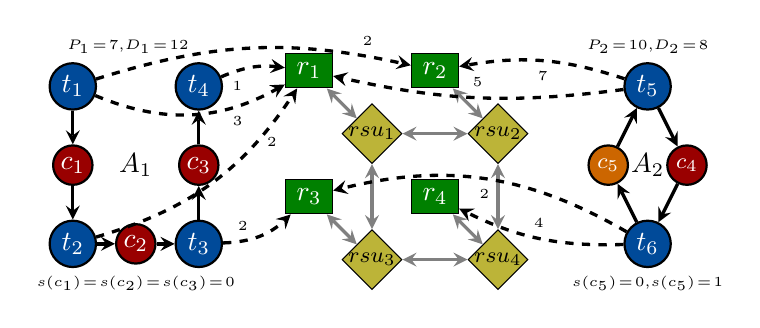
\begin{tikzpicture}[>=stealth]
	\tikzstyle{axis} = [->, black, very thick]
	\tikzstyle{link} = [<->, black!50, very thick]
	\tikzstyle{task} = [anchor=west,shape=rectangle,thick,text=white,minimum height=0.5cm, draw=black, fill=myblue, align=center, rounded corners=2,inner sep=0]
	\tikzstyle{difftask} = [shape=circle,thick,text=white,minimum height=0.5cm, draw=black, fill=myblue, align=center,inner sep=2]
	\tikzstyle{router} = [diamond,draw,fill=black!30!yellow,inner sep=0]
	\tikzstyle{resource} = [rectangle,minimum width=0.6cm,minimum height=0.4cm,draw,fill=black!50!green,text=white]
	\tikzstyle{route} = [->,black,line width=1.5]
	\node [router] (v1) at (-3.8,2.4) {\footnotesize$rsu_1$};
	\node [router] (v2) at (-2.2,2.4) {\footnotesize$rsu_2$};
	\node [router] (v4) at (-3.8,0.8) {\footnotesize$rsu_3$};
	\node [router] (v5) at (-2.2,0.8) {\footnotesize$rsu_4$};
	
	\draw [link] (v1) edge (v2);
	\draw [link] (v1) edge (v4);
	\draw [link] (v2) edge (v5);
	\draw [link] (v4) edge (v5);
	
	\node [resource] (v10) at (-4.6,3.2) {$r_1$};
	\node [resource] (v11) at (-3,3.2) {$r_2$};
	\node [resource] (v13) at (-4.6,1.6) {$r_3$};
	\node [resource] (v14) at (-3,1.6) {$r_4$};
	
	\draw [link] (v10) edge (v1);
	\draw [link] (v11) edge (v2);
	\draw [link] (v13) edge (v4);
	\draw [link] (v14) edge (v5);
	
	\node [difftask] (t1) at (-0.3,3) {$t_5$};
	\node [difftask,fill=black!40!red,inner sep=0] (c1) at (0.2,2) {\footnotesize$c_4$};
	\node [difftask,fill=black!20!orange,inner sep=0] (c2) at (-0.8,2) {\footnotesize$c_5$};
	\node [difftask] (t2) at (-0.3,1) {$t_6$};
	
	\draw [axis] (t1) edge (c1);
	\draw [axis] (c1) edge (t2);
	
	\draw [axis,dashed] (t2) edge[bend right=22] node[midway,below]{\tiny$2$}(v13);
	\draw [axis,dashed] (t2) edge[bend left=14] node[midway,above]{\tiny$4$}(v14);
	\draw [axis,dashed] (t1) edge[bend left=10] node[midway,above]{\tiny$5$}(v10);
	\draw [axis,dashed] (t1) edge[bend right=14] node[midway,below]{\tiny$7$}(v11);
	
	%\draw [route,black!40!red](v10) -- (-4.6,2.9) -- (-4.1,2.4) -- (-4.1,0.8) -- (-3.8,0.5) -- (-2.2,0.5)  --    (v14.south);
	%\draw [route,black!20!orange](v14.east) -- (-1.9,0.8) -- (-1.9,2.4) -- (-2.2,2.7) -- (-3.8,2.7)  --    (v10.east);
	\draw [axis] (t2) edge (c2);
	\draw [axis] (c2) edge (t1);
	\node[inner sep=0] at (-0.3,3.5) {\tiny $P_2=10, D_2=8$};
	\node[] at (-0.3,0.5) {\tiny $s(c_5)=0, s(c_5)=1$};
	
	\node [difftask] (t3) at (-7.6,3) {$t_1$};
	\node [difftask,fill=black!40!red,inner sep=0] (c3) at (-6,2) {$c_3$};
	\node [difftask,fill=black!40!red,inner sep=0] (c4) at (-7.6,2) {$c_1$};
	\node [difftask,fill=black!40!red,inner sep=0] (c5) at (-6.8,1) {$c_2$};
	\node [difftask] (t4) at (-6,1) {$t_3$};
	\node [difftask] (t5) at (-6,3) {$t_4$};
	\node [difftask] (t6) at (-7.6,1) {$t_2$};
	\draw [axis] (t3) edge (c4);
	\draw [axis] (c4) edge (t6);
	\draw [axis] (t6) edge (c5);
	\draw [axis] (c5) edge (t4);
	\draw [axis] (t4) edge (c3);
	\draw [axis] (c3) edge (t5);
	
	
	\draw [axis,dashed] (t3) edge[bend left=15] node[very near end,above]{\tiny$2$}(v11);
	\draw [axis,dashed] (t3) edge[bend right=26] node[near end,below]{\tiny$3$}(v10);
	\draw [axis,dashed] (t6) edge[bend right=20] node[near end,right]{\tiny$2$}(v10);
	\draw [axis,dashed] (t4) edge[bend right=21] node[near start,above]{\tiny$2$}(v13);
	\draw [axis,dashed] (t5) edge[bend left=15] node[near start,below]{\tiny$1$}(v10);
	\node[inner sep=0] at (-6.9,3.5) {\tiny $P_1=7, D_1=12$};
	\node[] at (-6.8,0.5) {\tiny $s(c_1)=s(c_2)=s(c_3)=0$};
	\node[] at (-0.3,2) {$A_2$};
	\node at (-6.8,2) {$A_1$};
\end{tikzpicture}
	\vspace*{-0.1cm}
	\caption{Specification example consisting of two applications $A_1$ and $A_2$, a $2\times 2$ platform template with four processing elements $p_{1-4}$ and routers $r_{1-4}$, and mapping options $m_1$ to $m_9$ annotated with WCET values. }
	\label{fig:specexample}
%	\vspace*{-0.1cm}
\end{figure}
%\vspace*{.5mm}
%\subsection{Architecture Template}

\textbf{Architecture Template: }
The architecture, or \emph{platform} template $P=(V_P,V_R,L)$ consists of processing elements $V_P$ and the communication infrastructure split into routers $V_R$ and links $L$. Both processing elements and routers are annotated by individual area and static power requirements that are used in the evaluation process to determine the quality of a solution. Additionally, the routing delay and energy determine the time and energy needed for each message to get send over one link. 
In this paper, we assume a circuit switching strategy for the routing of messages. That is, a message blocks the whole route from sender to receiver until it has been received completely. 
%However, each router internally consists of independent crossbar switches and corresponding input buffers to allow concurrent routing of messages if distinct links are involved in the communication. 
Note that bidirectional arrows represent two separate links. %For example, the connection between $p_1$ and $r_1$ in Fig.~\ref{fig:specexample} represents the directed edges $l_1=(p_1,r_1)$ and $l_2=(r_1,p_1)$.

%\vspace*{.5mm}
%\subsection{Specification Model}
\textbf{Problem Instance: }
For each task, a set of mapping options $M\subseteq T\times V_P$ is specified. A mapping option $m=(t,p)$ indicates that task $t$ may be executed on processing element $p$ and is annotated with a worst case execution time (WCET) as well as the dynamic energy consumed by $p$ when executing $t$. Specifying several mapping options per tasks with different WCETs and energy annotations corresponds to the modeling of heterogeneous systems.  Together with the applications and the platform template, the mapping options complete the problem instance $I=(A,P,M)$.\par

\textbf{Exploration Model: }
Acquiring a \emph{feasible} solution to the problem instance involves selecting a mapping for each task, routing the messages over the communication infrastructure, and determining a schedule while adhering to given timing constraints. Each solution is evaluated by three objective functions $latency$, $area$, and $energy$, that determine timing properties as well as area and energy requirements, respectively. These objective functions represent soft constraints that have to be optimized. Without loss of generality, the \ac{DSE} is formulated as a minimization problem as follows:
\begin{center}
	\vspace*{-0.1cm}
	\begin{minipage}[c]{0.2\textwidth}
		\begin{tabbing}
			mini\=mize $f(x) = (latency(x), area(x), energy(x)),$ \\
			subject to: \\
			\> $x$ is a feasible system implementation.
		\end{tabbing}
	\end{minipage}
	\vspace*{-0.1cm}
\end{center}
Here, a feasible system implementation is a solution that adheres to all given mapping, routing, and timing constraints. \par
In this work, we consider three different routing strategies. First, \emph{dimension order routing} (DOR) only allows one route for 
each pair of sending and receiving processing elements but simultaneously guarantees the shortest path. Second, \emph{shortest path 
routing} (SPR) also guarantees a shortest path between sender and receiver. However, the route is not fixed and various alternative 
routes can be selected. Finally, \emph{arbitrary length routing} (ALR) allows every acyclic route over the communication 
infrastructure and may be able to find solutions that distribute communication traffic over less congested links. That is, the 
number of decision variables and thus the complexity increases from DOR to ALR. 
\subsection{Answer Set Programming}
The specification model and the constraints described in the previous section are encoded as \acf{ASP} facts and rules. \ac{ASP} is 
a programming paradigm that is tailored towards NP-hard search problems and is based on the stable model (\emph{answer set}) 
semantics. Problems are formulated in a first-order input language as a set of facts and rules that are used to represent and infer 
domain knowledge, respectively. %Facts are the simplest constructs that are unconditionally true and consist of only one atom (i.e., an $n$-ary 
%predicate applied to $n$ terms). 
%Given the example in Fig.~\ref{fig:specexample}, the facts below encode the existence of task $t_1$ as well as its mapping options $m_1$ and $m_2$.
%\begin{equation}{\tt task(t1)}.\quad {\tt map(m1,t1,p1).}\quad {\tt map(m2,t1,p2).}\label{eq:facts}\end{equation}
%Rules are used to encode constraints. For example, the following (choice) rule encodes the selection mapping options. \begin{equation}\tt \{\ bind(M,T,P)\ :\ map(M,T,P)\ \} =1\ :-\ task(T).\label{eq:rules} \end{equation} 
%Here, the ternary predicate {\tt bind} (short {\tt bind/3}) is inferred exactly once for every {\tt task/1}. Thus, an answer set containing both {\tt bind(m1,t1,p1)} and {\tt bind(m2,t1,p2)} simultaneously cannot exist. Note that variables, indicated by capital letters, are used to provide a uniform problem definition that can be used for every specification instance.\par

Determining answer sets of logic programs (i.e., the combination of facts and rules) in \ac{ASP} is a two-step process. First, the
logic program is translated (\emph{grounded}) into a variable free representation before it can be solved by an answer set solver 
that determines stable models (\emph{solutions}). 
%Accordingly, grounding the example would result into $$\tt1\{bind(m1,t1,p1);bind(m2,t1,p2)\}1.$$
%Accordingly, solving the example in Eqs.~\ref{eq:facts} and \ref{eq:rules} produces two stable models (solutions): One with atom {\tt bind(m1,t1,p1)} and the other with {\tt bind(m2,t1,p2)}. 
The actual solving process is out of scope of this paper and we refer to \cite{gekakarosc15a} for further information.\par 
%To allow for optimizations of \ac{ASP} programs, \asprin{} %(\emph{ASP} for \emph{pr}eference handl\emph{in}g) 
%has been proposed in 
%\cite{Brewka2015} as a framework to compute preferred (optimal) solutions among stable models of logic programs based on 
%the solver \clingo. In addition to single-objective preference types, it also offers predefined 
%composite types like Pareto optimization.

Generally, \ac{ASP} is capable of finding stable models efficiently if there are only linear constraints involved. However, in system design, non-linear constraints such as timing requirements must be taken into account. To this end, we use \acf{ASPmT} (see~\cite{gekakaosscwa16a}) to incorporate custom background theories directly into the solving process. The details are displayed in the following section.%The coordination of \ac{ASP} and individual background theories is done with indicator variables that are known to both foreground and background theory. This way, conflicts that have been detected in the background theory are propagated to \ac{ASP} that subsequently prunes the search space accordingly. In this paper, we utilize \ac{QF--IDL} to analyze timing properties (see~\cite{Neubauer2017} for detailed information) as well as additional Pareto filters that are responsible for dominance checks. The details are described in the following section.


%\asprin{} (\emph{ASP} for \emph{pr}eference handl\emph{in}g) has been proposed in \cite{Brewka2015} as a framework to define and 
%compute preferred (optimal) solutions among stable models of logic programs. In addition to single-objective preference types such 
%as cardinality minimization, it also offers predefined composite (i.e.~multi-objective) preference types like Pareto optimization. 
%As \asprin{} is based on the \ac{ASP} solver \clingo{} \cite{gekakaosscwa16a}, it is only efficient for linear constraints. In this 
%work, we propose an optimization framework to \clingo{} that utilizes the input language of \asprin{} and allows non-linear 
%preference types. Therefore, we integrate background theories that handle both non-linear constraints solving and Pareto filtering. 









\section{Optimization Framework}
\label{sec:framework}
In this section, we present our novel system-level \acf{DSE} framework for finding Pareto optimal solutions. It utilizes the \ac{ASPmT} paradigm to evaluate non-linear objectives and performs dominance checks of feasible design points in individual background theories. In the following, an overview of our framework is given before various exact optimization strategies are presented. %Finally, an algorithmic description of our proposed approach is given.

%In the following, we present a general framework for calculating optimal solutions of ASPmT programs with arbitrary preferences,
%such as sum minimization or Pareto dominance.
%This framework allows for writing and including theories and preference types in \cpp\ as background propagators in a plug and play fashion
%and makes use of the \clingo\ \cpp\ API to implement an iterative solving process.
%We use this framework to, 
%first, implement two systems for optimizing preferences,
%one with preference types as background propagators only (\theory),
%and the other with preference types in ASP and as propagators (\hybrid),
%and second, we use both systems to calculate Pareto optimal solutions.

\subsection{Framework Overview}
%\begin{figure}
%\begin{adjustbox}{keepaspectratio, width=.5\textwidth}
%	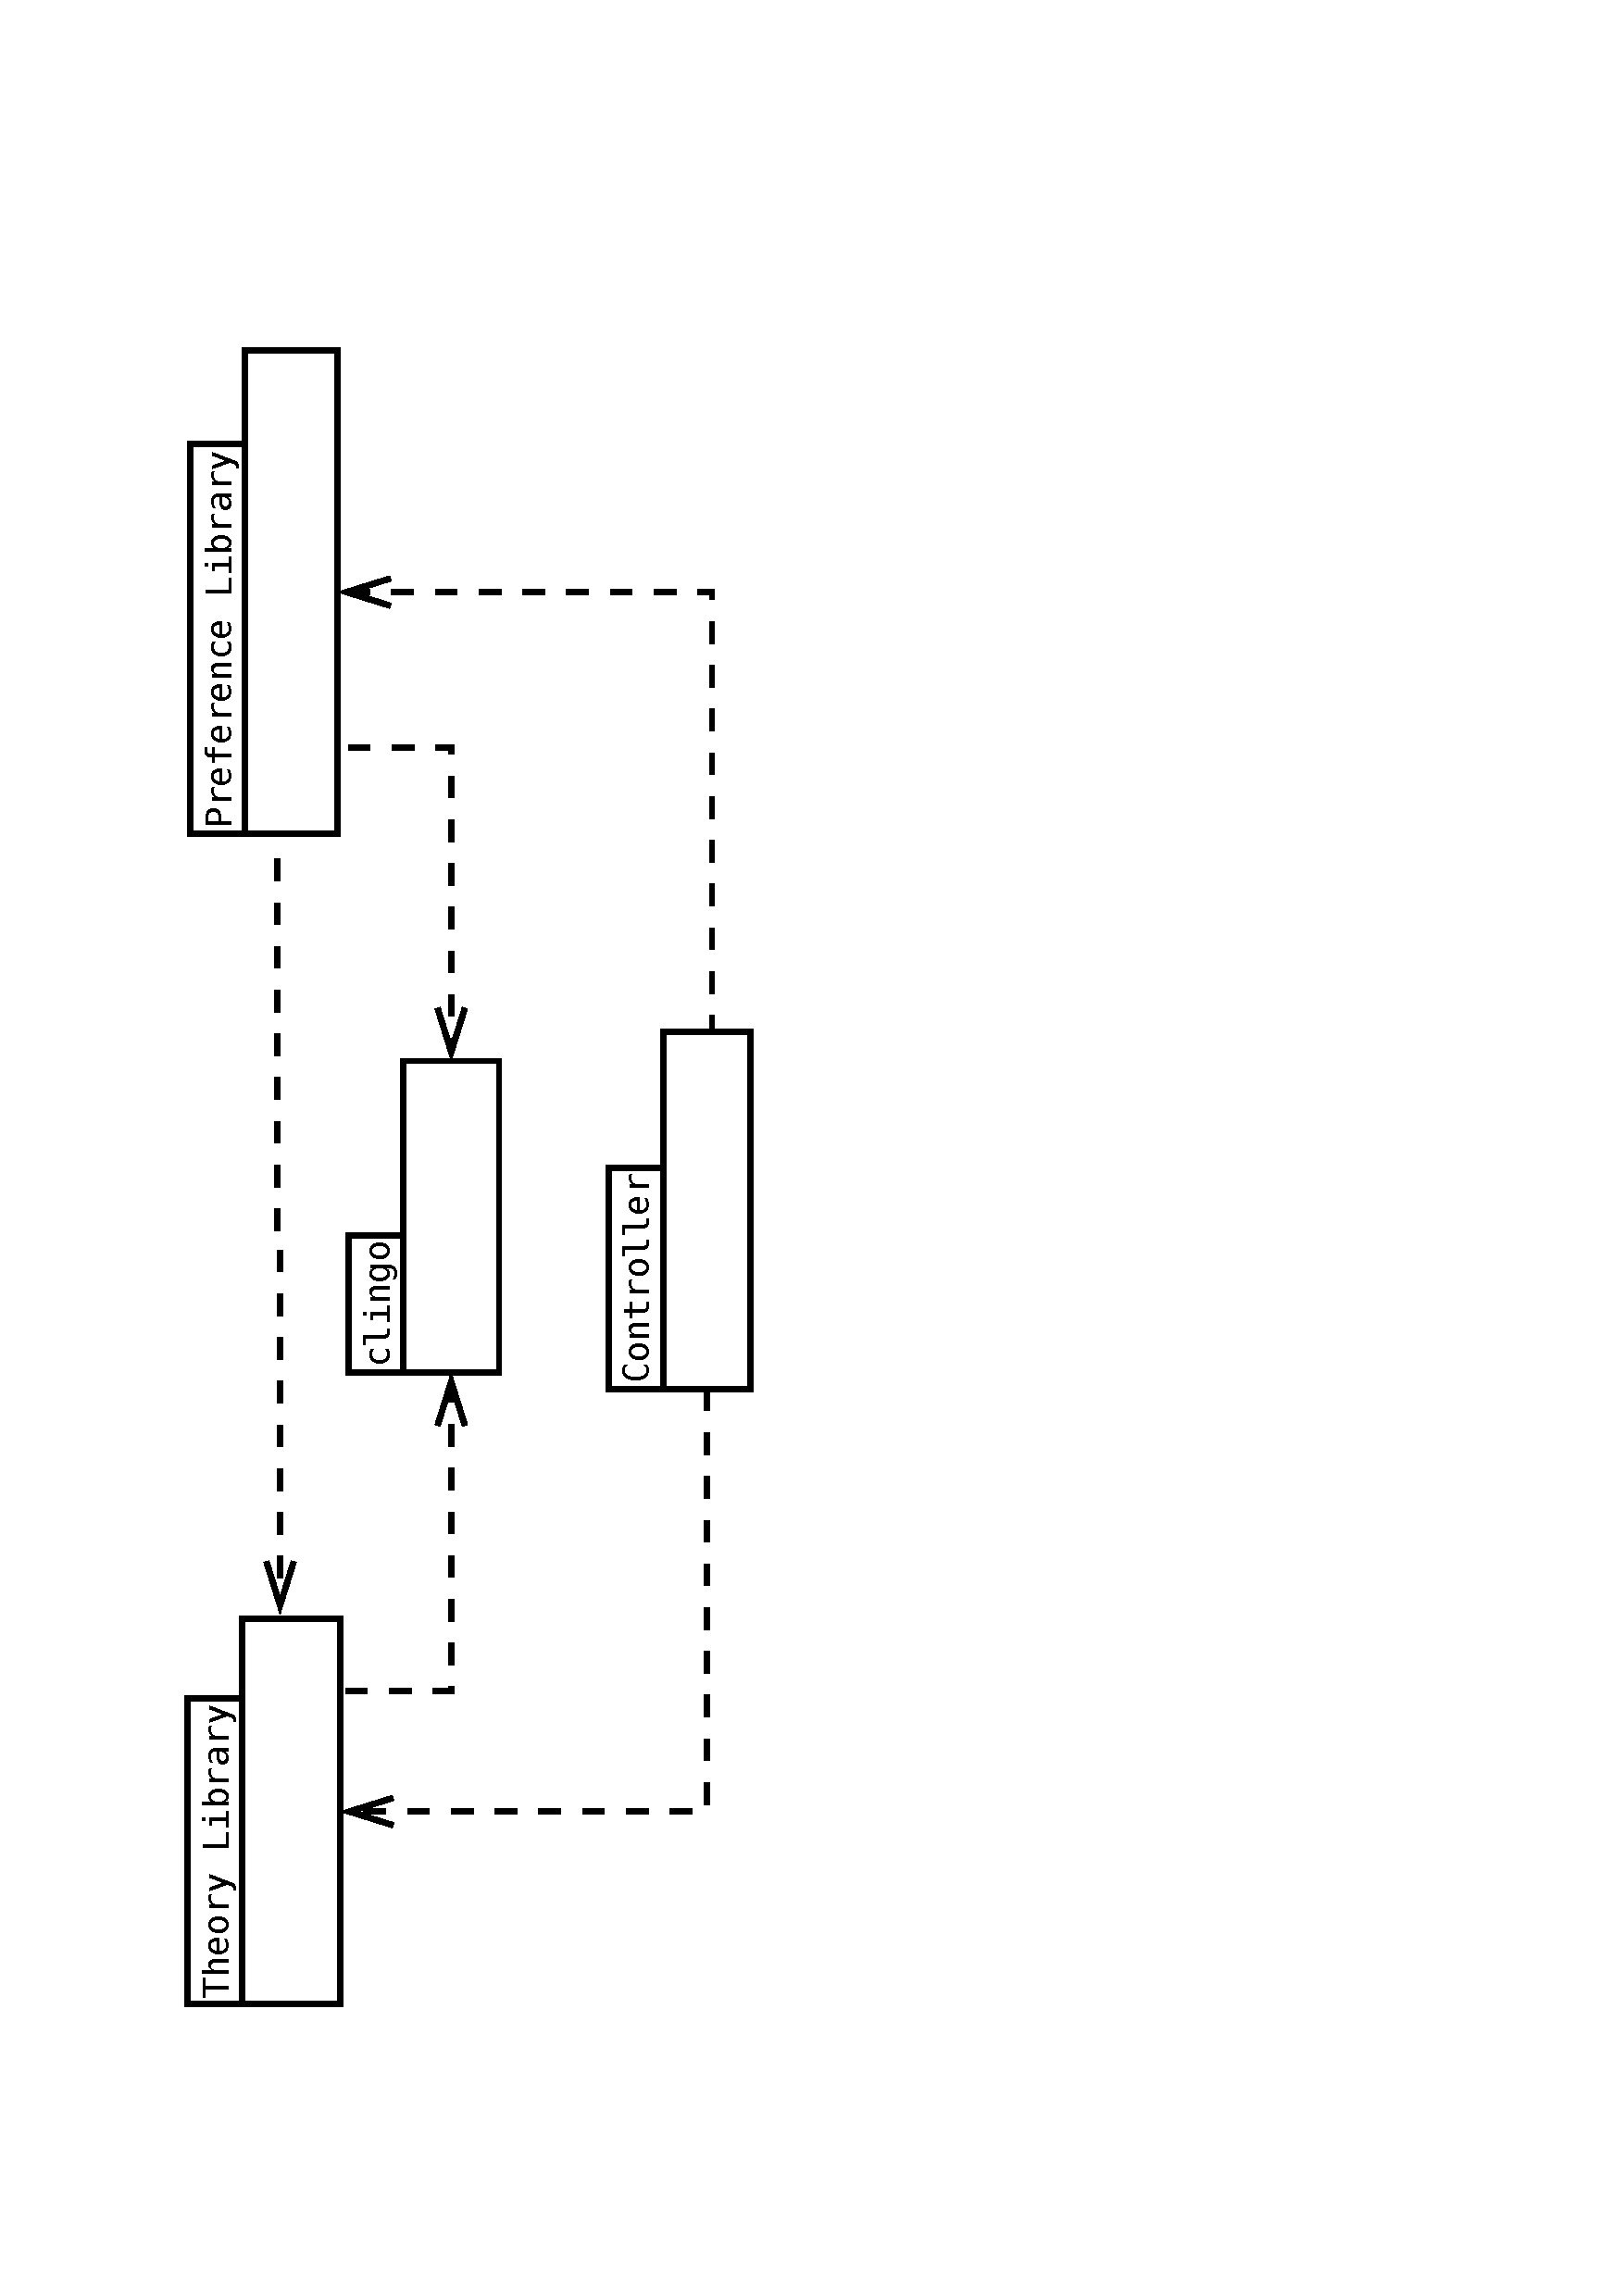
\includegraphics[angle=270, origin=c, height=\textheight]{architecture}
%\end{adjustbox}
%\vspace*{-5cm}
%\caption{Architecture of the ASPmT preference framework}
%\label{fig:architecture}
%\vspace*{-0.6cm}
%\end{figure}
\label{sec:overview}

The general overview of our proposed \ac{DSE} is depicted in Fig.~\ref{fig:architecture} and essentially consists of three pillars - the \ac{ASP} solver \clingo, a theory and an optimization propagator. A problem instance $I$ as described in Sec.~\ref{sec:model} in conjunction with a uniform problem definition encoded as \ac{ASP} program serve as input for our framework. In a first step, the program is grounded into a variable free representation that can be processed by the \ac{ASP} solver module of \clingo. During solving, \clingo\ propagates and assigns \ac{ASP} variables. In each solving step, routing and mapping decisions are made by \clingo\ before the (possibly partial) assignment is relayed to the background theory propagator that evaluates the current decisions w.r.t.~the objectives \emph{latency}, \emph{area}, as well as \emph{energy} and checks if given timing constraints are met. Subsequently, the current solution is forwarded to the optimization propagator that checks if it is non-dominated w.r.t.~already found solution stored in an archive.\footnote{Partial solutions can be used for dominance checks iff the problem is assignment monotonous, i.e., an additional decision must not improve the evaluation.}  Both constraint and dominance checking steps directly return conflict clauses to the \ac{ASP} solver whenever the results are negative. Here, they are utilized to restrict the search space that results in backtracking of already performed decisions. Note that this procedure is applied to partial assignments, i.e., incomplete solutions where not all decisions have been made, to prune infeasible and dominated regions early from the search. \par 
While partial assignments that pass constraint and dominance checks are handed back to \clingo, complete solutions trigger an archive update, i.e., adding the current and removing dominated design points. Furthermore, a conflict clause is propagated to the ASP solver to avoid visiting the same design point multiple times.\par 
Note that the system synthesis problem, i.e., acquiring a feasible binding, routing, and schedule, has to be solved for every design point considered in the \ac{DSE}. To this end, we utilize an \ac{ASPmT} approach as presented in \cite{Neubauer2017} that makes mapping and routing decisions in \ac{ASP} and leverages \ac{QF--IDL} as background theory to guarantee compliance to timing constraints. 
\begin{figure}
	\centering
	\resizebox{0.8\linewidth}{!}{\definecolor{myblue}{HTML}{004A99}
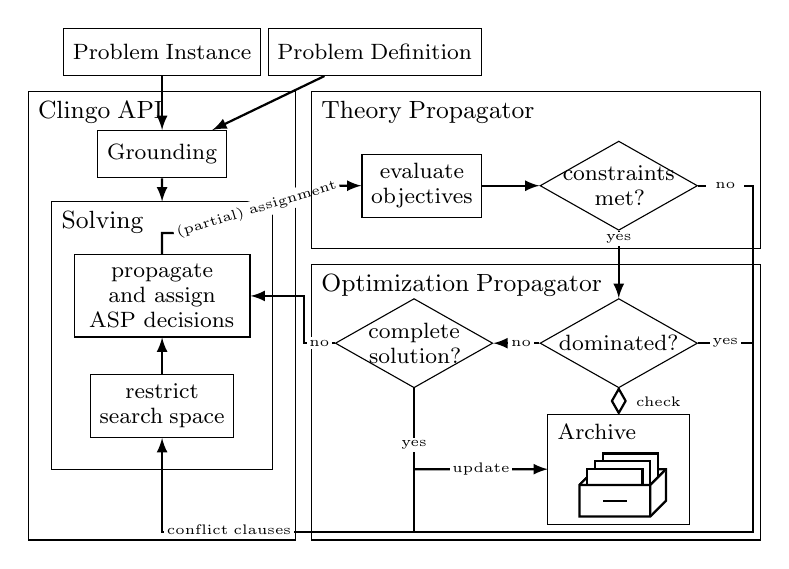
\begin{tikzpicture}
\tikzstyle{axis} = [-latex, thick]
\tikzstyle{link} = [<->, black!50, very thick]
\tikzstyle{task} = [anchor=west,shape=rectangle,thick,text=white,minimum height=0.5cm, draw=black, fill=myblue, align=center, rounded corners=2,inner sep=0]
\tikzstyle{difftask} = [shape=circle,thick,text=white,minimum height=0.5cm, draw=black, fill=myblue, align=center,inner sep=2]
\tikzstyle{router} = [icon,draw,fill=black!30!yellow,inner sep=0,minimum width=0.45cm,minimum height =0.3cm]
\tikzstyle{resource} = [rectangle,minimum width=0.6cm,minimum height=0.4cm,draw,fill=black!50!green,text=white]
\tikzstyle{route} = [->,black,line width=1.5]

\tikzstyle{textfield} = [draw,minimum height = 0.6cm,font=\footnotesize,text width=2cm,align=center]
\tikzstyle{decision} =[draw,diamond,text width=1.7cm,aspect=1.5,inner sep=0,align=center,font=\footnotesize,minimum width=2cm]
\node [textfield,text width=,] (v3) at (-1.4,-2.6) {Problem Instance};
\node [textfield,text width=,] (v80) at (1.3,-2.6) {Problem Definition};
\node [textfield,text width=] (v9) at (-1.4,-3.9) {Grounding};

%\draw [axis] (v4.west) --node[sloped,above=-3,font=\tiny]{depends on} (v3);

\coordinate (v5) at (-3.1,-3.1) {} {} {};
\coordinate (v6) at (-3.1,-8.8) {} {} {} {} {};
\coordinate (v7) at (0.3,-8.8) {} {} {} {} {} {};
\coordinate (v8) at (0.3,-3.1) {} {} {} {};
\draw  (v5) -- (v6) -- (v7) -- (v8) -- cycle;
\node[anchor = north west,font=\small] at (v5) {Clingo API};
\coordinate (s1) at (-2.8,-4.5) {} {} {} {} {} {} {};
\coordinate (s2) at (-2.8,-7.9) {} {} {} {} {} {} {} {};
\coordinate (s3) at (0,-7.9) {} {} {} {} {} {} {};
\coordinate (s4) at (0,-4.5) {} {} {} {} {} {};
\draw[] (s1) -- (s2) -- (s3) -- (s4) --node[midway] (smid){}  cycle;
\node [anchor=north west,font=\small] (s10) at (s1) {Solving};
\draw[axis]  (v3) edge (v9);
\draw[axis]  (v9) edge (smid.center);
\node [textfield,] (s9) at (-1.4,-5.7) {propagate and assign ASP decisions};



\coordinate (a1) at (0.5,-5.3) {} ;
\coordinate (a2) at (0.5,-8.8) {} {} {} {} {} ;
\coordinate (a3) at (6.2,-8.8) {} {} {} {} {} {} {} {} {} ;
\coordinate (a4) at (6.2,-5.3) {} {} {} {} {} {} {} ;
\draw  (a1) -- (a2) -- (a3) -- (a4) -- cycle;
\node[anchor = north west,font=\small] at (a1) {Optimization Propagator};
\node [textfield,minimum width=0cm,text width=,] (x3) at (1.9,-4.3) {evaluate\\objectives};

\coordinate (v1) at (-1.4,-4.9) {} {} {} {} {};
\coordinate (v2) at (-1.2,-4.9) {} {} {} {} {} {} {} {} {} {};
\coordinate (v4) at (0.8,-4.3) {} {} {} {} {} {} {} {} {};
\draw[axis]  (s9) -- (v1)--(v2)--node[midway,sloped,,font=\tiny,fill=white,inner sep=1,outer sep=1]{(partial) assignment}(v4)-- (x3);

\node [decision] (v10) at (4.4,-4.3) {};
\node[font=\footnotesize,text width=2cm,align=center] at (v10) {constraints\\met?};
\draw[axis]  (x3) -- (v10);
\node [decision] (v11) at (4.4,-6.3) {};
\node[font=\footnotesize] at (v11) {dominated?};
\draw[axis]  (v10) --node[very near start, ,fill=white,font=\tiny,inner sep=1,outer sep=1]{yes}  (v11);
\node [decision] (v12) at (1.8,-6.3) {};
\node[font=\footnotesize,text width=2cm,minimum width=1,align=center] at (v12) {complete\\solution?};
\draw [axis] (v11) --node[pos=0.4, sloped,fill=white,font=\tiny,inner sep=1,outer sep=1]{no}  (v12);

\node [textfield,minimum width=0cm,text width=,fill=white] (v13) at (-1.4,-7.1) {restrict\\search space};
\draw [axis] (v13) edge (s9);
%\draw [axis] (v10) --node[midway, sloped,fill=white,font=\tiny,inner sep=0,outer sep=0]{conflict clause} (v13);
%\draw [axis] (v11) --node[midway, sloped,fill=white,font=\tiny,inner sep=0,outer sep=0]{conflict clause} (v13);
\coordinate (v40) at (0.4,-6.3) {} {} {} {} {} {} {} {};
\draw [axis] (v12) --node[midway, sloped,fill=white,font=\tiny,inner sep=1,outer sep=1]{no} (v40)|-(s9);



\coordinate (v17) at (3.9,-8.5) {} {} {} {} {} {} {} {} {} {} {} ;
\coordinate (v18) at (4.8,-8.5) {} {} {} {} {} {} {} {} {} {} {} ;
\coordinate (v16) at (3.9,-8.1) {} {} {} {} {} {} {} {} {} {} ;
\coordinate (v21) at (4.8,-8.1) {} {} {} {} {} {} {} {} {} {} ;
\coordinate (v22) at (5,-8.3) {} {} {} {} {} {} {} {} {} {} {} ;
\coordinate (v15) at (5,-7.9) {} {} {} {} {} {} {} {} {} {} {}  ;
\coordinate (v14) at (4.1,-7.9) {} {} {} {} {} {} {} {} {} {} ;
\coordinate (v19) at (4.2,-8.3) {} {} {} {} {} {} {} {} {} {} ;
\coordinate (v20) at (4.5,-8.3) {} {} {} {} {} {} {} {} {} {} ;
\coordinate (v24) at (4.7,-7.9) {} {} {} {} {} {} {} {} {} {} {} ;
\coordinate (v25) at (4.7,-8.1) {} {} {} {} {} {} {} {} {} {} {} {} ;
\coordinate (v26) at (4.8,-7.8) {} {} {} {} {} {} {} {} {} {} {}  ;
\coordinate (v27) at (4.1,-7.8) {} {} {} {} {} {} {} {} {} {} {} ;
\coordinate (v28) at (4,-8.1) {} {} {} {} {} {} {} {} {} {} ;
\coordinate (v29) at (4,-7.9) {} {} {} {} {} {} {} {} {} {} ;
\coordinate (v30) at (4.1,-8.1) {} {} {} {} {} {} {} {} {} {} {} ;
\coordinate (v31) at (4.9,-7.7) {} {} {} {} {} {} {} {} {} {} {} {} ;
\coordinate (v32) at (4.9,-8.1) {} {} {} {} {} {} {} {} {} {} {} {} {} ;
\coordinate (v33) at (4.2,-8.1) {} {} {} {} {} {} {} {} {} {} {} ;
\coordinate (v34) at (4.2,-7.7) {} {} {} {} {} {} {} {} {} {} {} ;
\draw[thick]  (v14) edge (v16);
\draw[thick]  (v14) edge (v15);
\draw[thick,fill=white]  (v16) -- (v17) -- (v18) -- (v22) -- (v15) -- (v14) -- cycle;
\draw [thick,fill=white] (v31) -- (v32)--(v33) --(v34) --cycle;
\draw[thick,fill=white] (v26)--(v27) -- (v30) -- (v21) -- cycle;
\draw [thick,fill=white] (v29) -- (v28)--(v25) --(v24) --cycle;
\draw [thick] (v15)--(v21) -- (v16);
\draw [thick,fill=white] (v18) -- (v21)--(v15);

%\draw[thick,fill=white]  (v16) -- (v17) -- (v18) -- (v22) -- (v15) -- (v14) -- cycle;
%\draw[thick,fill=white]  (v18) -- (v22) -- (v15) -- (v21) --cycle;
\draw [thick] (v19) -- (v20);
\coordinate (v38) at (1.8,-7.9) {} {} {} {} {} {} {} {} {} {};
\coordinate (v39) at (1.8,-8.7) {} {} {} {} {} {} {} {} {} {};
\draw [axis,-] (v12) --node[midway,fill=white,font=\tiny,pos=0.7,inner sep=1,outer sep=1,align=center]{yes} (v38) -- (v39);
\coordinate (v23) at (3.5,-7.2) {} {} {} {} {} {} {};
\coordinate (v37) at (5.3,-7.2) {} {} {} {} {} {} {};
\coordinate (v35) at (3.5,-8.6) {} {} {} {} {} {} {} {} {};
\coordinate (v36) at (5.3,-8.6) {} {} {} {} {} {} {};
\draw [] (v23) --node[midway](archleft){} (v35) --node[midway](archmid){} (v36) --node[midway](archright){} (v37) --node[midway](archtop){} cycle;
\node[anchor = north west,font=\footnotesize] at (v23) {Archive};



\draw [axis] (v38) --node[midway, sloped,fill=white,font=\tiny,inner sep=1,outer sep=1,align=center]{update} (archleft.center);% -- (archleft.center);
%\draw [axis] (v38) --node[midway, sloped,fill=white,font=\tiny,inner sep=0,outer sep=0]{conflict clause} (v13);

\draw[axis,open diamond-,dashed] (archtop.center)--node[midway, right=0.15,fill=white,font=\tiny,inner sep=1,outer sep=1,align=center]{check}(v11);%--node[midway, sloped,fill=white,font=\tiny,inner sep=0,outer sep=0,align=center]{check}(v11);
\coordinate (v41) at (6.1,-4.3) {} {} {};
\coordinate (v42) at (6.1,-6.3) {} {} {};
\coordinate (v45) at (6.1,-8.7) {} {} {} {} {};
\coordinate (v43) at (0.3,-8.7) {} {} {} {};
\coordinate (v44) at (-1.4,-8.7) {} {} {};
\draw [axis](v10) --node[fill=white,font=\tiny]{no} (v41) -- (v42)--(v45) -- (v43) --node[midway,,above=-0.1, sloped,fill=white,font=\tiny,inner sep=1,outer sep=1]{conflict clauses} (v44) -- (v13);
\draw [axis,-] (v11) --node[midway,sloped,pos=0.5,font=\tiny,fill=white,inner sep=1,outer sep=1]{yes} (v42);
%\draw [thick] (v38) edge (v44);
\coordinate (v47) at (0.5,-5.1) {};
\coordinate (v48) at (6.2,-5.1) {} {};
\coordinate (v49) at (6.2,-3.1) {} {} {};
\coordinate (v46) at (0.5,-3.1) {} {};
\draw (v46) -- (v47) -- (v48) -- (v49) -- cycle;
\node[anchor = north west,font=\small] at (v46) {Theory Propagator};
\draw [axis] (v80) -- (v9);
\end{tikzpicture}}
	\vspace*{-0.1cm}
	\caption{Architecture of the ASPmT optimization framework}
	\label{fig:architecture}
%	\vspace*{-0.1cm}	
\end{figure}
\subsection{Optimization Strategies}
To the best of our knowledge, this work presents for the first time a system-level \ac{DSE} executed in a background theory of a symbolic constraint solver. However, with \asprin\ \cite{Brewka2015}, a general framework for preference handling has been developed that supports multi-objective optimization of linear objectives. Therefore, our first \ac{DSE} strategy is similar to \asprin\ but with the extension of additional background theory propagators in order to support non-linear constraint solving. %Thus, we call this approach \emph{hybrid} in the following. 
%To this end, we develop three different strategies for executing the \ac{DSE}. 
As it is based on the combination of \asprin\ with background theories, we call it the \emph{hybrid} approach in the following. Here, linear objectives are calculated and the dominance checks are performed directly by the solver while background theories are only utilized to evaluate design points w.r.t.~non-linear objectives. This strategy adds constraints to the problem definition ensuring an improvement of a solution compared to the previous one or the incomparability to already obtained Pareto optimal solutions. As a consequence, only after a design point is proven to be located on the true Pareto front, incomparable design points can be found. Hence, the convergence of the approximation set towards the Pareto front contains a \emph{depth-first} characteristic. As is common in \ac{ASP}, previous stable models are partly saved via facts within the logic program rendering an explicit archive in a background theory obsolete. \par
In contrast to the first \hybrid\ strategy, our second one utilizes background theory propagators for both evaluation and dominance checks. Similar to \hybrid, it follows a \emph{depth-first} characteristic. Consequently, this strategy is called \emph{theory\textsubscript{depth}} in the following. The archive of the optimization propagator saves all found Pareto optima as well as the current design point that is guaranteed to be incomparable to them. Hence, the current approximation set can be obtained at any time. \par
Finally, \emph{theory\textsubscript{breadth}} again makes use of the dominance check in the Pareto propagator and thus, contains the current approximation set. In contrast to \emph{theory\textsubscript{depth}}, design points are not strictly required to dominate the previously found solution but rather the archive is also updated whenever an incomparable design point w.r.t.~the whole approximation set is found. The possible advantage of this strategy is two fold. First, diverse design points may be obtained more frequently as novel non-dominated solutions are added independent of the previously found design point. Second, as a consequence, the dominance check step has more information on dominated regions of the design space which allows for a more efficient pruning in early steps of the decision process. However, the convergence of the approximation set towards the true Pareto front may be slower as the solving is not primarily directed to prove Pareto optimality of found solutions.\footnote{As all the presented methods are exact, the Pareto optimality is proven inherently after all possible decisions have been made.} 
%\begin{itemize}
%	\item Notion of an Optimal solution differs
%	\item \theory = The whole pareto front is an optimal solution
%	\item \hybrid = One Pareto optimal design point is an optimal solution
%\end{itemize}
%\subsection{Optimization Algorithm}
%\begin{algorithm}[t!]
%	\footnotesize
%	%\small
%	\caption{Branch-and-bound style algorithm}
%	\label{algo:bb}
%	\SetAlgoVlined
%	\KwIn{problem instance $I$, ASPmT problem definition $E$,\newline number of optimal solutions $n$}
%	$GP \gets \mathtt{GROUND}(E\cup I)$\;
%	$TO,PO \gets \mathtt{INSTANTIATE}(\mathtt{ANALYZE}(GP))$\;
%	$o \gets 0;\text{ }i \gets 0;\text{ }\mathcal{S} \gets \emptyset$; $\mathit{unsat}\gets \mathit{False}$\;
%	\While{$True$}{
%		$\mathit{ret}\gets\mathtt{SOLVE}(GP,TO,PO)$\;
%		\eIf {$\mathit{ret} = \mathit{Unsatisfiable}$}{
%			\If {$i=0$ {\bf or} $\mathit{unsat}$}{
%				\Return{$\mathcal{S}$}\;
%			}
%			$\mathcal{S}\gets \mathcal{S} \cup \mathtt{GET\_SOLUTION}(i)$\;    	
%			$o=o+1$\;
%			\If{$o=n$}{
%				\Return{$\mathcal{S}$}\;
%			}
%			$\mathit{unsat}\gets \mathit{True}$\;
%			$\mathtt{REMOVE\_COMPARE\_SOLUTION}(GP,PO,i)$\;
%			$\mathtt{OPTIMUM\_FOUND}(GP,PO,i)$\;
%		}
%		{
%			$\mathit{unsat}\gets \mathit{False}$\;
%			$i=i+1$\;
%			$\mathtt{SAVE\_SOLUTION}(ret,i)$\;
%			\If{$i>1$}{
%				$\mathtt{REMOVE\_COMPARE\_SOLUTION}(GP,PO,i-1)$\;
%			}
%			$\mathtt{ADD\_COMPARE\_SOLUTION}(GP,PO,i)$\;
%		}
%	}
%\end{algorithm}	
%The two systems, \theory\ and \hybrid, use variations of Algorithm~\ref{algo:bb}.
%In essence, the branch-and-bound algorithm computes a solution,
%then tries to find a better one,
%and repeats this process until no further solution can be found, 
%thus proving the last solution to be optimal.
%Algorithm~\ref{algo:bb} receives an ASPmT problem definition $E$, 
%an instance $I$ and a desired number of optimal solution $n$
%and returns a set of maximum $n$ optimal solutions. Note that the notion of an optimal solution differs between \theory\ and \hybrid\ strategies. While for \theory\, an optimal solution equates the true Pareto front as a whole, \hybrid\ considers each Pareto optimal design point to be an optimal solution.
%
%The algorithm first grounds the combined logic program of $E$ and $I$ (Line~1).
%The optimization parameters contained in the resulting ground program $GP$ are analyzed,
%and the necessary theory $TO$ and optimization background propagators $PO$ are instantiated (Line~2).
%After initialization of the state variables, viz. current number of optimal solutions $o$, number of solutions found $i$,
%set of optimal solutions $\mathcal{S}$ and Boolean variable $\mathit{unsat}$ to indicate unsatisfiabilty, the main loop starts by trying to find a new solution (Line~6). That is, as described in Sec.~\ref{sec:overview}, the ground logic program is solved by the \ac{ASP} solver while constraint and dominance checks are constituted in the background theory propagators $TO$ and $PO$, respectively.\par
%The returned value of one solving call equates either to \emph{Unsatisfiable} or contains a solution that is better than the previous one and incomparable to already found optimal solutions. In the former case, i.e., if no solution could be found (lines~7--16), three possibilities arise: first, the original problem is unsatisfiable, viz. $i=0$,
%second, it was proven that no further optimal solutions exist, viz. $\mathit{unsat}=\mathit{True}$,
%and third, a new optimal solution was found. In the first two cases, the algorithm stops and the set of optimal solutions $\mathcal{S}$ is returned (Line~9).
%In the latter case, solution $i$ is optimal and is added to $\mathcal{S}$ and the number of optimal solutions $o$ is incremented by one.
%If $o$ equals $n$, the desired number of optimal solutions is returned.
%To save the information that no intermediate solution has been found yet, $\mathit{unsat}$ is set to $\mathit{True}$.
%Since the recent solving step could not find a new solution that is better than solution $i$,
%the comparison to solution $i$ is removed from the ground program and the optimization propagator (Line~15).
%Subsequently, program and optimization propagator are configured to ensure that every subsequent model is incomparable to solution $i$ (Line~16).
%
%\vspace*{-0.1cm}In case a new solution is found,
%$\mathit{unsat}$ is set to $\mathit{False}$,
%and the solution counter $i$ is increased by one (lines~18--19).
%The new solution is saved under identifier $i$ (Line~20).
%If there has been a previous intermediate solution,
%the comparison to it is removed from optimization propagator and ground program (Line~21) and the novel solution becomes the optimal solution candidate (Line~22). 
%After that, the main loop starts anew by trying to compute the next (better) solution.\par
%
%Accordingly, the algorithm either computes the desired number of optimal solutions or proves that there exist less than $n$.
%Note that the algorithm is exact and complete.
%Given enough time, all optimal models are computed and proven to be optimal.
%As this is often unrealistic in practice, we allow for interrupting the algorithm at any point and return the currently best known approximation set, viz. solution $i$ and the set $\mathcal{S}$. 
%
%Note that the solving step (line 6) supports all of \clingo's sophisticated solving modes
%including domain-specific heuristics \cite{Andres2015} and multi-threading \cite{gekakarosc15a}. While domain specific heuristics help in diminishing the overall runtime of the algorithm, multiple threads are used to set up the solver with different configurations in each thread that leads to varying approaches for covering the decision space.
%In case a new solution is found,
%$\mathit{unsat}$ is set to $\mathit{False}$,
%and solution counter $i$ is increased by one (lines~18--19).
%The new solution is saved under identification number $i$ (Line~20).
%If there has been a previous intermediate solution, the comparison to it is removed from the optimization objects and the ground program (Line~21).
%To ensure that the next solution is better, a comparison is added between the new solution and solution $i$ (Line~22). 
%After that, the main loop starts anew by trying to compute the next solution.
%
%If $i$ is 0, this amounts to finding a random solution to the ground program $GP$ that is consistent with the theories in $TO$.
%For $i$ greater 0, the ground program and the preferences $PO$ ensure 
%that the new solution is better than the previous one and incomparable to all previous optimal solutions.
%Elements of $TO$ and $PO$ are background propagators~\cite{gekakaosscwa16a} that are called during solving to ensure that the current partial assignment is,
%first, consistent with the theories,
%and second, not worse than the previous solution.
%Note that such solve calls supports all of \clingo's sophisticated solving modes
%including domain-specific heuristic~\cite{Andres2015} and multi-threading~\cite{gekakarosc15a}.

%If no solution could be found (lines~8--16),
%three possibilities arise:
%first, the original problem is unsatisfiable, viz. $i=0$,
%second, it was proven that no further optimal solutions, viz. $\mathit{unsat}=\mathit{True}$,
%and third, a new optimal solution was found.
%In the first two cases, the algorithm stops and the set of optimal solutions $\mathcal{S}$ is returned (Line~9).
%In the latter case, solution $i$ is optimal and is added to $\mathcal{S}$ and $o$ is incremented by one.
%If $o$ equals $n$, the desired number of optimal solutions is returned.
%To save the information that no intermediate solution has been found yet, $\mathit{unsat}$ is set to $\mathit{True}$.
%Since the recent solving step required the new solution to be better than solution $i$ 
%which was not possible,
%the comparison to solution $i$ is removed from ground program and preferences (Line~15).
%Following that, program and preferences are configured to ensure that every subsequent model is incomparable to solution $i$ (Line~16).

  
%\subsection{title}
%
%Figure~\ref{fig:architecture} depicts the basic architecture of the optimization framework.
%At the center is the \clingo\ \cpp\ API that provides methods for grounding, solving, and accessing ASPmT programs.
%Besides that, \texttt{Theory Library} and \texttt{Preference Library} are modules that
%enable the user to write and include theories and preference types, respectively,
%into their system (here denoted by a generic controller module) in a general manner.
%Note that \texttt{Preference Library} depends on \texttt{Theory Library} 
%since a preference type may need to access a theory, 
%as is the case for the preference type \emph{latency} 
%which requires the variable assignments provided by the QF-IDL theory.
%
%\subsection{Preference types}
%
%A core concept of the framework are so-called \emph{preference types}.
%A preference type defines whether a solution is \emph{better, equal}, or \emph{worse} than another solution.
%In the following, we describe the preference types we use in the context of our application.
%
%\paragraph{sum}
%The \emph{sum} preference type assigns integer values to certain attributes of a solution,
%and compares the sum of those values for which the attributes hold.
%A solution is \emph{better} if the sum is lower.
%
%\paragraph{latency}
%The \emph{latency} preference type is defined over a set of tasks, 
%and compares the maximum of the sum of start and current execution time of those tasks,
%i.e. the latest point of execution.
%A solution is \emph{better} if the value is lower.
%
%\paragraph{paretoDepth}
%The \emph{paretoDepth} preference type aggregates an arbitrary number of other preferences,
%and the comparison amounts to Pareto dominance,
%i.e. a solution is \emph{better} then another if all underlying preferences are at least as good and one is strictly better.
%For example, assuming two quantitative preferences where lower is better,
%$(2,0)$ is better than $(3,1)$.
%
%\paragraph{paretoBreadth}
%The \emph{paretoBreadth} preference type is similar to the \emph{paretoDepth} preference,
%but here the comparison is extended to sets of incomparable solutions.
%Given two sets of solutions $S_1$ and $S_2$,
%$S_1$ is \emph{better} than $S_2$,
%if $S_1$ can be obtained by removing dominated solutions from $S_1\cup S_2$,
%and $S_1$ contains one non-dominated solution not in $S_2$.
%For example, assuming two quantitative preferences where lower is better,
%$\{(0,3),(2,0)\}$ is better than $\{(0,3),(3,1),(2,2)\}$.
%This type was devised to simultaneously collect non-dominated solutions,
%and remove previous dominated solutions,
%to get closer to the Pareto front step by step.
%
%\subsection{Preference Specification}
%A \emph{preference specification} declares what specific instances of preference types are used and what preference is optimized.
%We call the preference that is optimized \emph{lead preference}.
%As is common in ASP(mT), this is done in a declarative fashion that allows for flexibility and rapid changes.
%For brevity, we will not give a formal definition but rather explain the preference specification used for the application at hand.
%Given an instance of the specification model $I=(A,P,M)$ and an architecture template $P=(V_P,V_R,L)$, 
%we device the preference specification as follows:
%\paragraph{latency}
%We define a preference of type \emph{latency} over all tasks in $A$.
%Which mapping in $M$ was chosen in the solution determines the WCET,
%and the schedule, provided by the QF-IDL theory, determines the start time.
%\paragraph{area}
%We define a preference of type \emph{sum}.
%As attributes we consider every possible processing element, router or link in $P$
%that might be allocated either by having a task mapped onto or message routed over it,
%and declare as value the individual area that is annotated.
%\paragraph{energy}
%We define a preference of type \emph{sum}.
%For the static power, we consider every possible processing element or router in $P$
%that might be allocated either by having a task mapped onto or message routed over it,
%and declare as value the individual static power that is annotated times the period.
%For the dynamic energy, every possible instance of a link in $L$ being used is considered as an attribute,
%as well as the possible mappings from $M$ that might be chosen, 
%both with the respective annotated dynamic energy consumption as value.
%\paragraph{optimization}
%As the lead preference we declare either a preference of type \emph{paretoDepth} or \emph{paretoBreadth},
%which in turn aggregate preferences \emph{latency}, \emph{area} and \emph{energy}. 
%Note that enumerating all optimal solutions regarding \emph{paretoDepth} as well as obtaining one optimal solution of \emph{paretoBreadth} calculates the whole Pareto front.
%
%
%\subsection{Systems}
%\subsubsection{Algorithm}	
%
%	
%The two systems, \theory\ and \hybrid, use variations of Algorithm~\ref{algo:bb}.
%In essence, the branch-and-bound algorithm computes a solution,
%then tries to find a better one regarding the lead preference,
%and repeats this process until no further solution can be found, 
%thus proving the last solution to be optimal.
%Algorithm~\ref{algo:bb} receives an ASPmT encoding $E$, 
%a preference specification $P$, 
%an instance $I$ and a desired number of optimal solution $n$
%and returns a set of maximum $n$ optimal solutions.
%
%The algorithm first grounds $E$, $I$ together with $P$ (Line~1).
%The preference specification contained in the resulting ground program $GP$ is analyzed,
%and the needed theories $TO$ and preferences $PO$ are instantiated (Line~2).
%After initialization of the needed variables, 
%viz. current number of optimal solutions $o$,
%number of solutions found $i$,
%set of optimal solutions $\mathcal{S}$ 
%and Boolean variable $\mathit{unsat}$ to indicate unsatisfiabilty,
%the main loop starts by trying to find a new solution (Line~6).
%If $i$ is 0, this amounts to finding a random solution to the ground program $GP$ that is consistent with the theories in $TO$.
%For $i$ greater 0, the ground program and the preferences $PO$ ensure 
%that the new solution is better than the previous one and incomparable to all previous optimal solutions.
%Elements of $TO$ and $PO$ are background propagators~\cite{gekakaosscwa16a} that are called during solving to ensure that the current partial assignment is,
%first, consistent with the theories,
%and second, not worse than the previous solution.
%Note that such solve calls supports all of \clingo's sophisticated solving modes
%including domain-specific heuristic~\cite{Andres2015} and multi-threading~\cite{gekakarosc15a}.
%
%If no solution could be found (lines~8--16),
%three possibilities arise:
%first, the original problem is unsatisfiable, viz. $i=0$,
%second, it was proven that no further optimal solutions, viz. $\mathit{unsat}=\mathit{True}$,
%and third, a new optimal solution was found.
%In the first two cases, the algorithm stops and the set of optimal solutions $\mathcal{S}$ is returned (Line~9).
%In the latter case, solution $i$ is optimal and is added to $\mathcal{S}$ and $o$ is incremented by one.
%If $o$ equals $n$, the desired number of optimal solutions is returned.
%To save the information that no intermediate solution has been found yet, $\mathit{unsat}$ is set to $\mathit{True}$.
%Since the recent solving step required the new solution to be better than solution $i$ 
%which was not possible,
%the comparison to solution $i$ is removed from ground program and preferences (Line~15).
%Following that, program and preferences are configured to ensure that every subsequent model is incomparable to solution $i$ (Line~16).
%
%In case that a new solution is found,
%$\mathit{unsat}$ is set to $\mathit{False}$,
%and solution counter $i$ is increased by one (lines~18--19).
%The new solution is saved under identification number $i$ (Line~20).
%If there has been a previous intermediate solution,
%the comparison to it is removed from preferences and ground program (Line~21).
%To ensure that the next solution is better regarding the lead preference, 
%a comparison is added between the new solution and solution $i$ (Line~22). 
%After that, the main loop starts anew by trying to compute the next solution.
%
%Accordingly, the algorithm either computes the desired number of optimal solutions or proves that there exist less than $n$.
%Note that the algorithm is exact and complete.
%Given enough time, all optimal models can be computed and are proven to be optimal.
%In practice, this is often unrealistic,
%which is why we allow for interrupting the algorithm at any point and return the currently best known solution, viz. solution $i$ and the set $\mathcal{S}$.

%\subsubsection{\theory}
%
%This variation of the algorithm relies on one preference propagator to ensure that the next solution is better than the current solution.
%The propagator receives one \emph{assignment monotone} lead preference to be optimized.
%A preference is assignment monotone if for every partial assignment, 
%the quality remains equal or deteriorates if the assignment is extended.
%On a partial assignment, the propagator checks, 
%whether the current quality is already worse than the previous solution,
%in which case the solver excludes the partial assignment, and all assignments containing it,
%and jumps to a different area of the search space.
%The propagator requires a full assignment to be better than the recent intermediate solution,
%and incomparable to all previous optimal ones, 
%otherwise it rejects the assignment.
%Note that previous solutions are saved in the preference objects in their entirety,
%and, even though only one answer set may be added per iteration,
%the currently best known or optimal solution may consist of several answer sets,
%e.g. for preference type \emph{paretoBreadth}
%
%\subsubsection{\hybrid}
%
%The hybrid approach extends the methodology of \asprin\ by being able to add preference types in \cpp\ and include background theories like QF-IDL.
%Here, ASP rules are added to ensure that the next answer set improves on the previous one,
%or is incomparable to already obtained optimal solutions.
%Every preference is registered as a propagator and handles determining the truth value of predefined interface variables signifying whether two models are better, worse or equal. 
%Since the enumeration mechanism relies on partly saving previous answer sets via facts in the logic program,
%there is a one to one correspondence between solution and answer set.


\section{Conclusion}\label{conclusion}

We presented an ASP-based approach for solving the 
curriculum-based course timetabling (CB-CTT) problems.
The resulting system {\asap}~\footnote{%
All source code is available from %
\texttt{https://potassco.org/doc/apps/}}
is built upon general-purpose ASP systems, in our case {\clingo}.
That is, {\asap} relies on high-level ASP encodings presented in
Section~\ref{sec:approach}, \ref{sec:ext}, and \ref{mpp}
and delegates both the grounding
and solving tasks to {\clingo}.

The main features of our declarative approach are as follows:
%
\begin{list}{}{}
\item \textbf{Expressiveness}. 
The expressive power of ASP's modelling language enables us to compactly express
a wide variety of hard and soft constraints of CB-CTT as demonstrated
by a collection of {\asap} encodings. 
Given new constraints (e.g., Manhattan distance), 
all we have to do is adding ASP rules.

\item \textbf{Flexibility}. 
{\asap} provides flexible lexicographic optimization and easy
composition of different formulations, since any combination of
constraints can be represented as ASP facts. 
Consequently, it enables a timetable keeper to experiment with
different formulations as well as to optimize the obtained timetable 
with different priority levels of soft constraints, 
at a purely declarative level.

\item \textbf{Efficiency}. 
Our empirical analysis considers all instances in five different 
formulations, which are publicly available from the CB-CTT portal. 
% Many instances are based on real world data from several European
% universities. 
We have contrasted the performance of \asap\ with the best known
bounds obtained so far via more dedicated implementations.
\asap\ demonstrated that our declarative approach allows us to
compete with state-of-the-art CB-CTT solving techniques.

\item \textbf{Scalability}. 
The optimized encoding drastically reduces the grounding time compared
to the basic encoding.
Consequently, our declarative approach scales to large instances in
complex formulations, as demonstrated by the fact that
{\asap} was able to find upper bounds for very
large instances in the category \code{erlangen} with every
formulation, and 24 of them were unsolvable before. 

\item \textbf{Extensibility}. 
The high-level approach of ASP facilitates extensions and variations
of first-order encodings.
From this viewpoint, 
we extended the {\asap} system to solving multi-objective course
timetabling problem combining CB-CTT and minimal perturbation problems
with two criteria of optimality and stability.
\end{list}

Perhaps the most relevant related works are problem encodings in Integer Programming%
~\citep{%
      DBLP:journals/cor/BurkeMPR10,%
      DBLP:journals/anor/BurkeMPR10,%
      DBLP:journals/anor/BurkeMPR12,%
      DBLP:journals/anor/LachL12}.
These encodings use the binary variables $x_{C,D,P}$ and/or
$x_{C,R,D,P}$ that correspond to the predicate
\code{assigned/3} and/or \code{assigned/4} respectively.
SAT/MaxSAT encodings~\citep{DBLP:journals/aicom/AchaN12} also 
use the same binary variables.
%
The major advantage of our approach is not only
the compact and flexible declarative representation gained by using
ASP as a modeling language,
but also the high performance gained from the recent advanced
techniques in ASP solving.

Our ASP-based approach can be applied to a wide range of timetabling
problems such as
\textit{school timetabling},
\textit{examination timetabling}, and
\textit{post-enrollment course timetabling}.
Multi-objective optimization implemented in \asap\ can be further
extended in selecting a promising subset of Pareto optimal solutions
by using an advanced technique in MODOP solving based on P-minimal
model generation~\citep{sbtl2017}.
%
ASP-based large neighborhood search (LNS) for course timetabling can
be promising
because a MaxSAT-based LNS has been recently shown to be effective for
high school timetabling~\citep{DBLP:journals/cor/DemirovicM17}.
For this, we developed a prototype implementing a simple neighborhood
search using multi-shot ASP solving with {\asap}.
In a preliminary experiment on some \code{comp} instances in UD5, 
the prototype was able to find new bounds for 
 33 for \code{comp10},
135 for \code{comp13},
142 for \code{comp09}, and
143 for \code{comp21}.
%
We will investigate these possibilities, and 
the results will be applied to representing and reasoning more
practical timetabling problems.

%%% Local Variables:
%%% mode: latex
%%% TeX-master: "paper"
%%% End:



\section*{Acknowledgment}
This work was funded by the German Science Foundation (DFG) under grants HA 4463\slash4-1 and SCHA 550/11-1.
%Blinded for review.
\footnotesize
\bibliographystyle{unsrt}
\bibliography{library}%,lit,akku,procs}





% trigger a \newpage just before the given reference
% number - used to balance the columns on the last page
% adjust value as needed - may need to be readjusted if
% the document is modified later
%\IEEEtriggeratref{8}
% The "triggered" command can be changed if desired:
%\IEEEtriggercmd{\enlargethispage{-5in}}

% references section

% can use a bibliography generated by BibTeX as a .bbl file
% BibTeX documentation can be easily obtained at:
% http://mirror.ctan.org/biblio/bibtex/contrib/doc/
% The IEEEtran BibTeX style support page is at:
% http://www.michaelshell.org/tex/ieeetran/bibtex/
%\bibliographystyle{IEEEtran}
% argument is your BibTeX string definitions and bibliography database(s)
%\bibliography{IEEEabrv,../bib/paper}
%
% <OR> manually copy in the resultant .bbl file
% set second argument of \begin to the number of references
% (used to reserve space for the reference number labels box)
%\begin{thebibliography}{1}
%
%\bibitem{IEEEhowto:kopka}
%H.~Kopka and P.~W. Daly, \emph{A Guide to \LaTeX}, 3rd~ed.\hskip 1em plus
%  0.5em minus 0.4em\relax Harlow, England: Addison-Wesley, 1999.
%
%\end{thebibliography}




% that's all folks
\end{document}
